\documentclass[]{report}

% Use utf-8 encoding for foreign characters
\usepackage[utf8]{inputenc}
% For euro symbol
\usepackage{eurosym}
% for http links
\usepackage[hidelinks]{hyperref}

% Setup for fullpage use
\usepackage{fullpage}
%\usepackage{graphicx}
%\usepackage{subfig}
%\usepackage{float}
%\usepackage{listings}

\usepackage[francais]{babel}

\usepackage{times}
%\usepackage{rotate}
%\usepackage{lscape}

\usepackage{color}
\usepackage{placeins}

\usepackage{forest}
\usepackage{amsmath}
\usepackage{amssymb}
\usepackage{algpseudocode}
\usepackage{graphicx}
\usepackage{subfiles}
\usepackage{geometry}


\makeatletter
\DeclareRobustCommand{\genericinterval}[2]{%
	\@ifstar{\genericinterval@star{#1}{#2}}{\genericinterval@nostar{#1}{#2}}}
\newcommand{\genericinterval@star}[4]{\mathopen{}\mathclose{\left#1#3:#4\right#2}}
\newcommand{\genericinterval@nostar}[4]{\mathopen{#1}#3:#4\mathclose{#2}}
\newcommand{\intervalcc}{\genericinterval[]}
\newcommand{\intervaloo}{\genericinterval][}
\newcommand{\intervaloc}{\genericinterval]]}
\newcommand{\intervalco}{\genericinterval[[}
\makeatother

\newcommand{\placeholder}[1]{{\noindent \color{red}[ #1 ]}}
\newcommand{\comp}[1]{\mathcal{O}(#1)}
\def\Li{\par\leavevmode\par}

\newcommand{\navbutton}[2]{Le bouton \emph{#1} : envoie l'utilisateur sur la fenêtre \emph{#2}}
\newcommand{\textfield}[2]{Le champ de texte \emph{#1} : permet à l'utilisateur d'entrer #2}
\newcommand{\passwordfield}[2]{Le champ de mot de passe \emph{#1} : permet à l'utilisateur d'entrer #2 de manière discrète}
\newcommand{\access}[1]{\ \\ \noindent\textbf{Accès} : #1 \\}
\newcommand{\content}[1]{\textbf{Contenu} : #1}

%-----Commandes pour page de garde UMons
\usepackage[fs]{umons-coverpage}
\umonsAuthor{
	Augustin \textsc{Houba} \\
	Arnaud \textsc{Moreau} \\
	Cyril \textsc{Moreau} \\
	François \textsc{Vion}
}
\umonsTitle{Rapport de modélisation du projet de Génie Logiciel}
\umonsSubtitle{S-INFO-015}
\umonsDocumentType{Rapport de modélisation\\
7 décembre 2021}
\umonsSupervisor{ \\
	Prof. Tom \textsc{Mens}\\
} 
% The date (or academic year)
\umonsDate{Année académique 2021-2022}

\begin{document}
%\tikzset
%	every label/.append style={font=\scriptsize},
%	my edge labels/.style={font=\scriptsize},
%	dominant/.append style={label=below:$dominant$},
%}
%\frontmatter          % for the preliminaries
%\pagestyle{headings}  % switches on printing of running heads
%\mainmatter              % start of the contributions

%\umonsCoverPage

\subfile{subfiles/Titlepage.tex}

\newpage

\tableofcontents

\newpage

\chapter{Introduction}

\newpage

\subfile{subfiles/Introduction.tex}

\newpage
\chapter{Partie commune}


\newpage




\section{Introduction et choix de conception des diagrammes de conception UML}



\subsection{Use case diagrams}
Les différentes descriptions semi-Structurée se trouvent dans un PDF attaché à ce rapport afin de garentir une certaine clarté dans ce rapport.
\newpage

\subsection{Interaction overview diagrams}

\subfile{subfiles/Interaction Overview Intro, Auth & Choix de conception.tex}

\newpage

\subsection{Class diagrams}

\subfile{subfiles/Intro class.tex}

\newpage

\subsection{Sequence diagrams}

\subfile{subfiles/Intro Sequence.tex}

\newpage




\section{Diagrammes de conception UML : application client}



\subsection{Use case diagram}

\subfile{subfiles/Use Case Client.tex}

\begin{figure}[h]
	\centering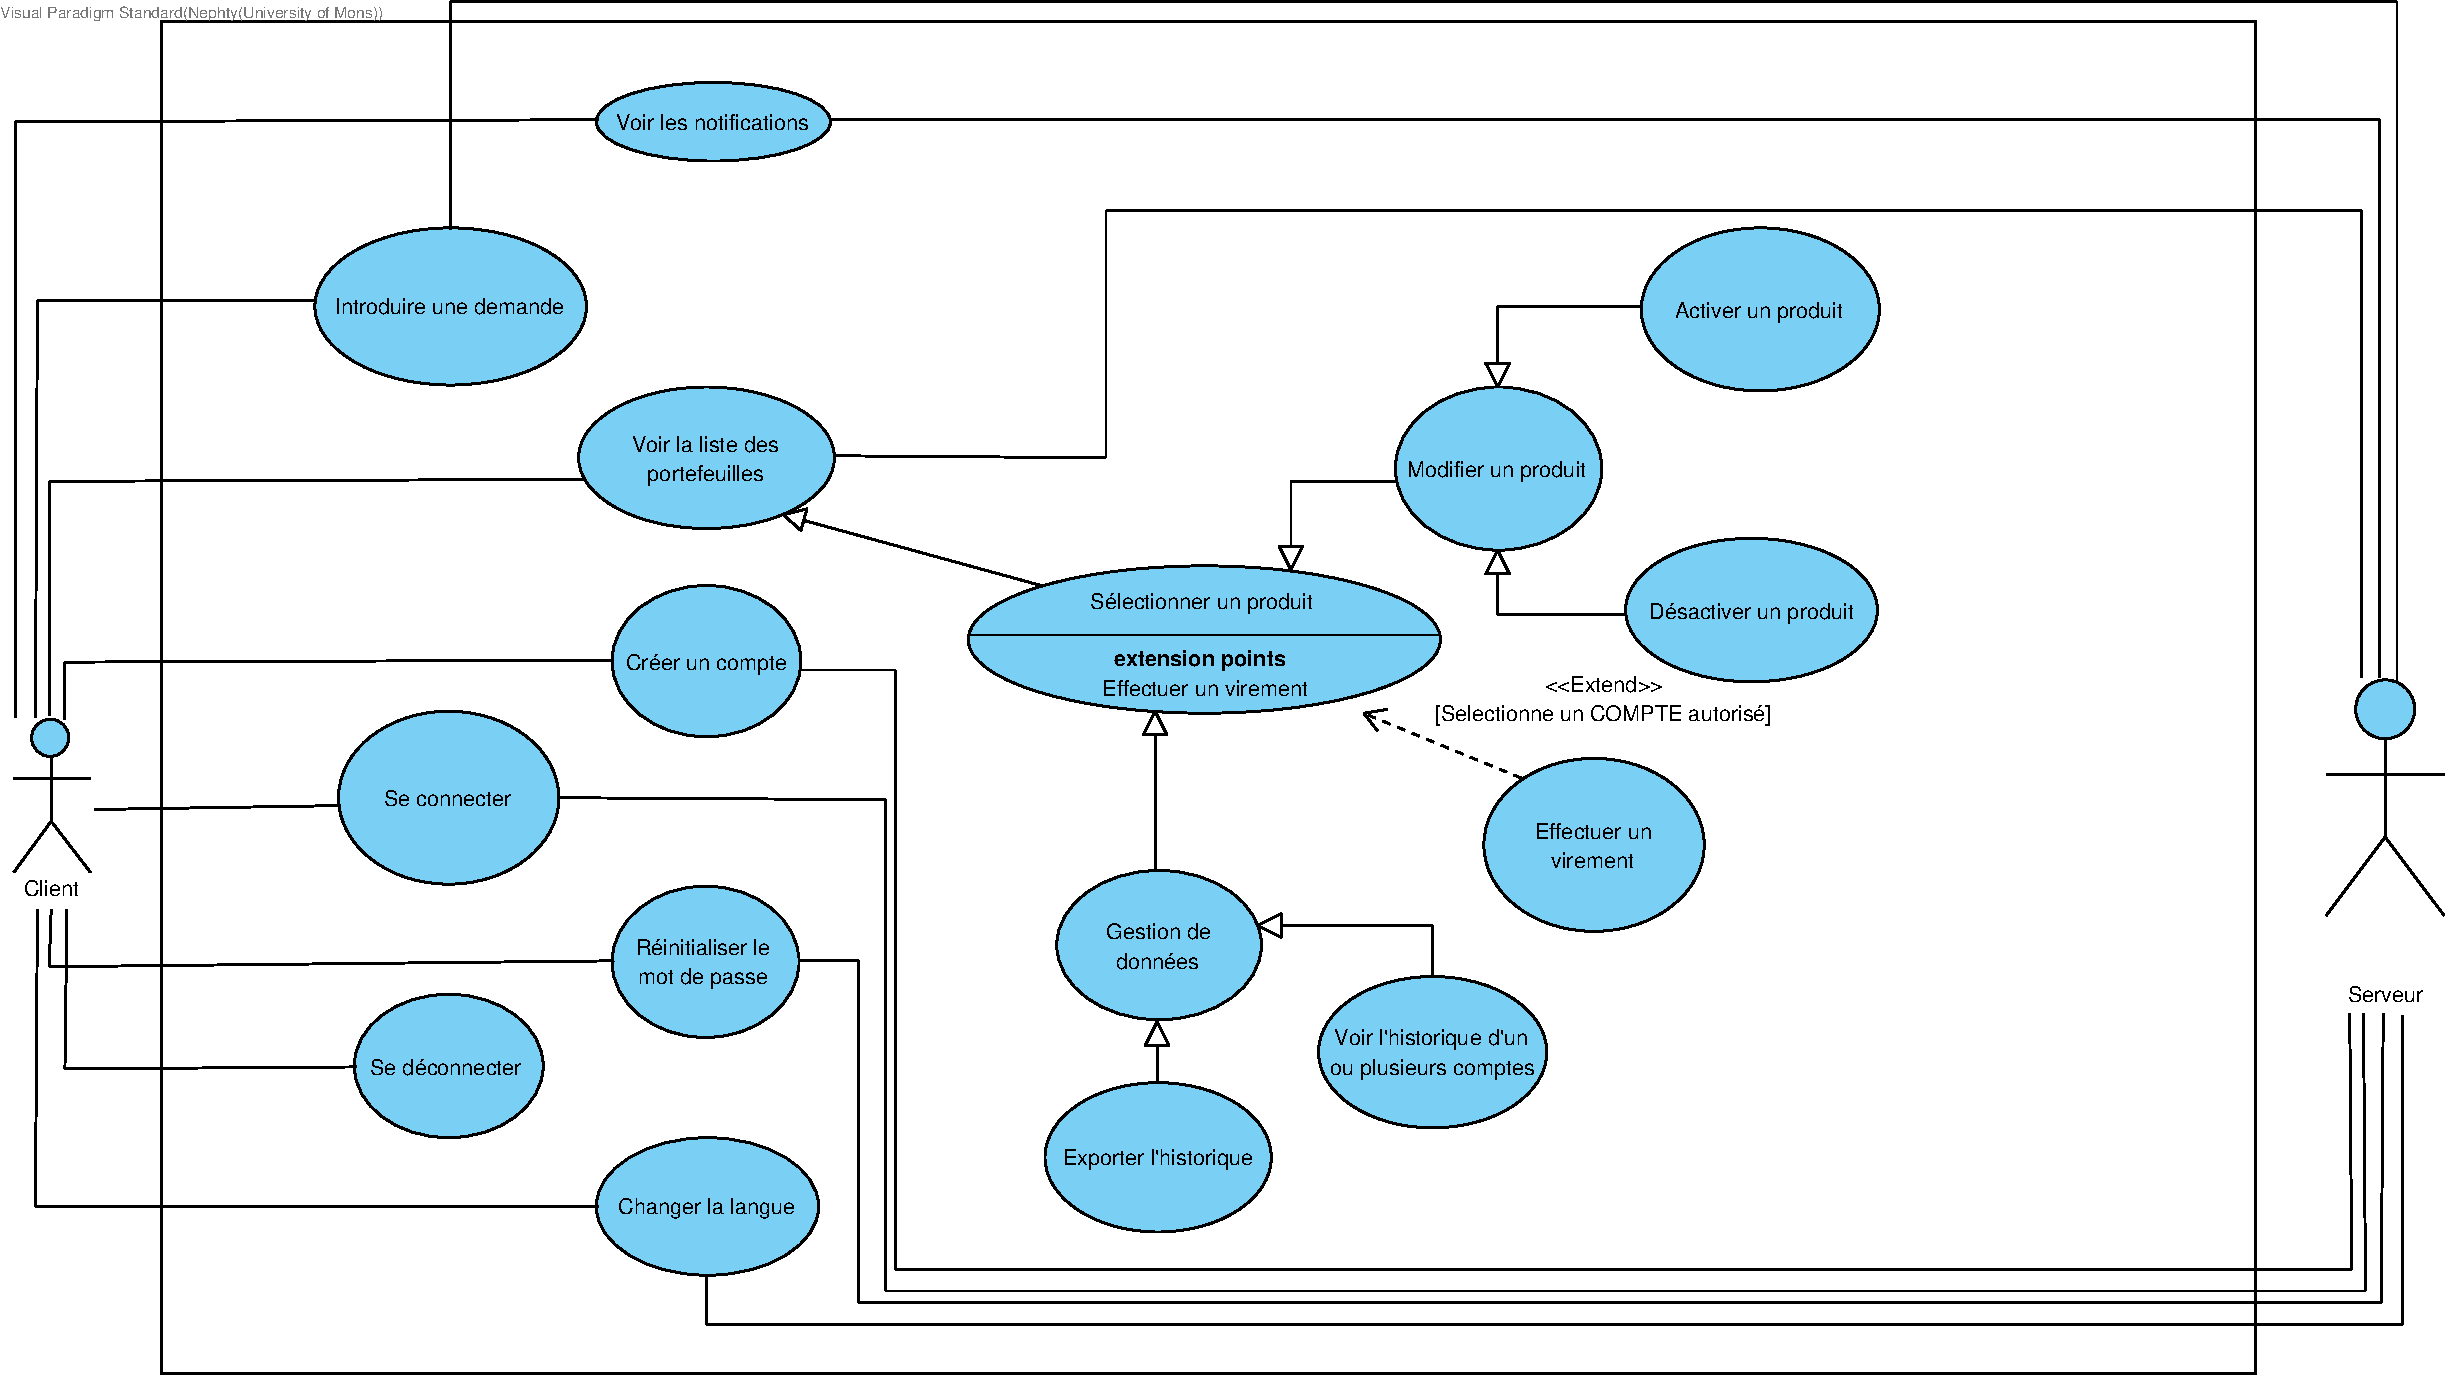
\includegraphics[width=\linewidth]{img/Use Case Client.pdf}
	\caption{Diagramme de case d'utilisation de l'application client.}
\end{figure}

\newpage

\subsection{Interaction overview diagram}

\subfile{subfiles/Interaction Overview Client.tex}

\begin{figure}[h!]
\hbox{
	\centering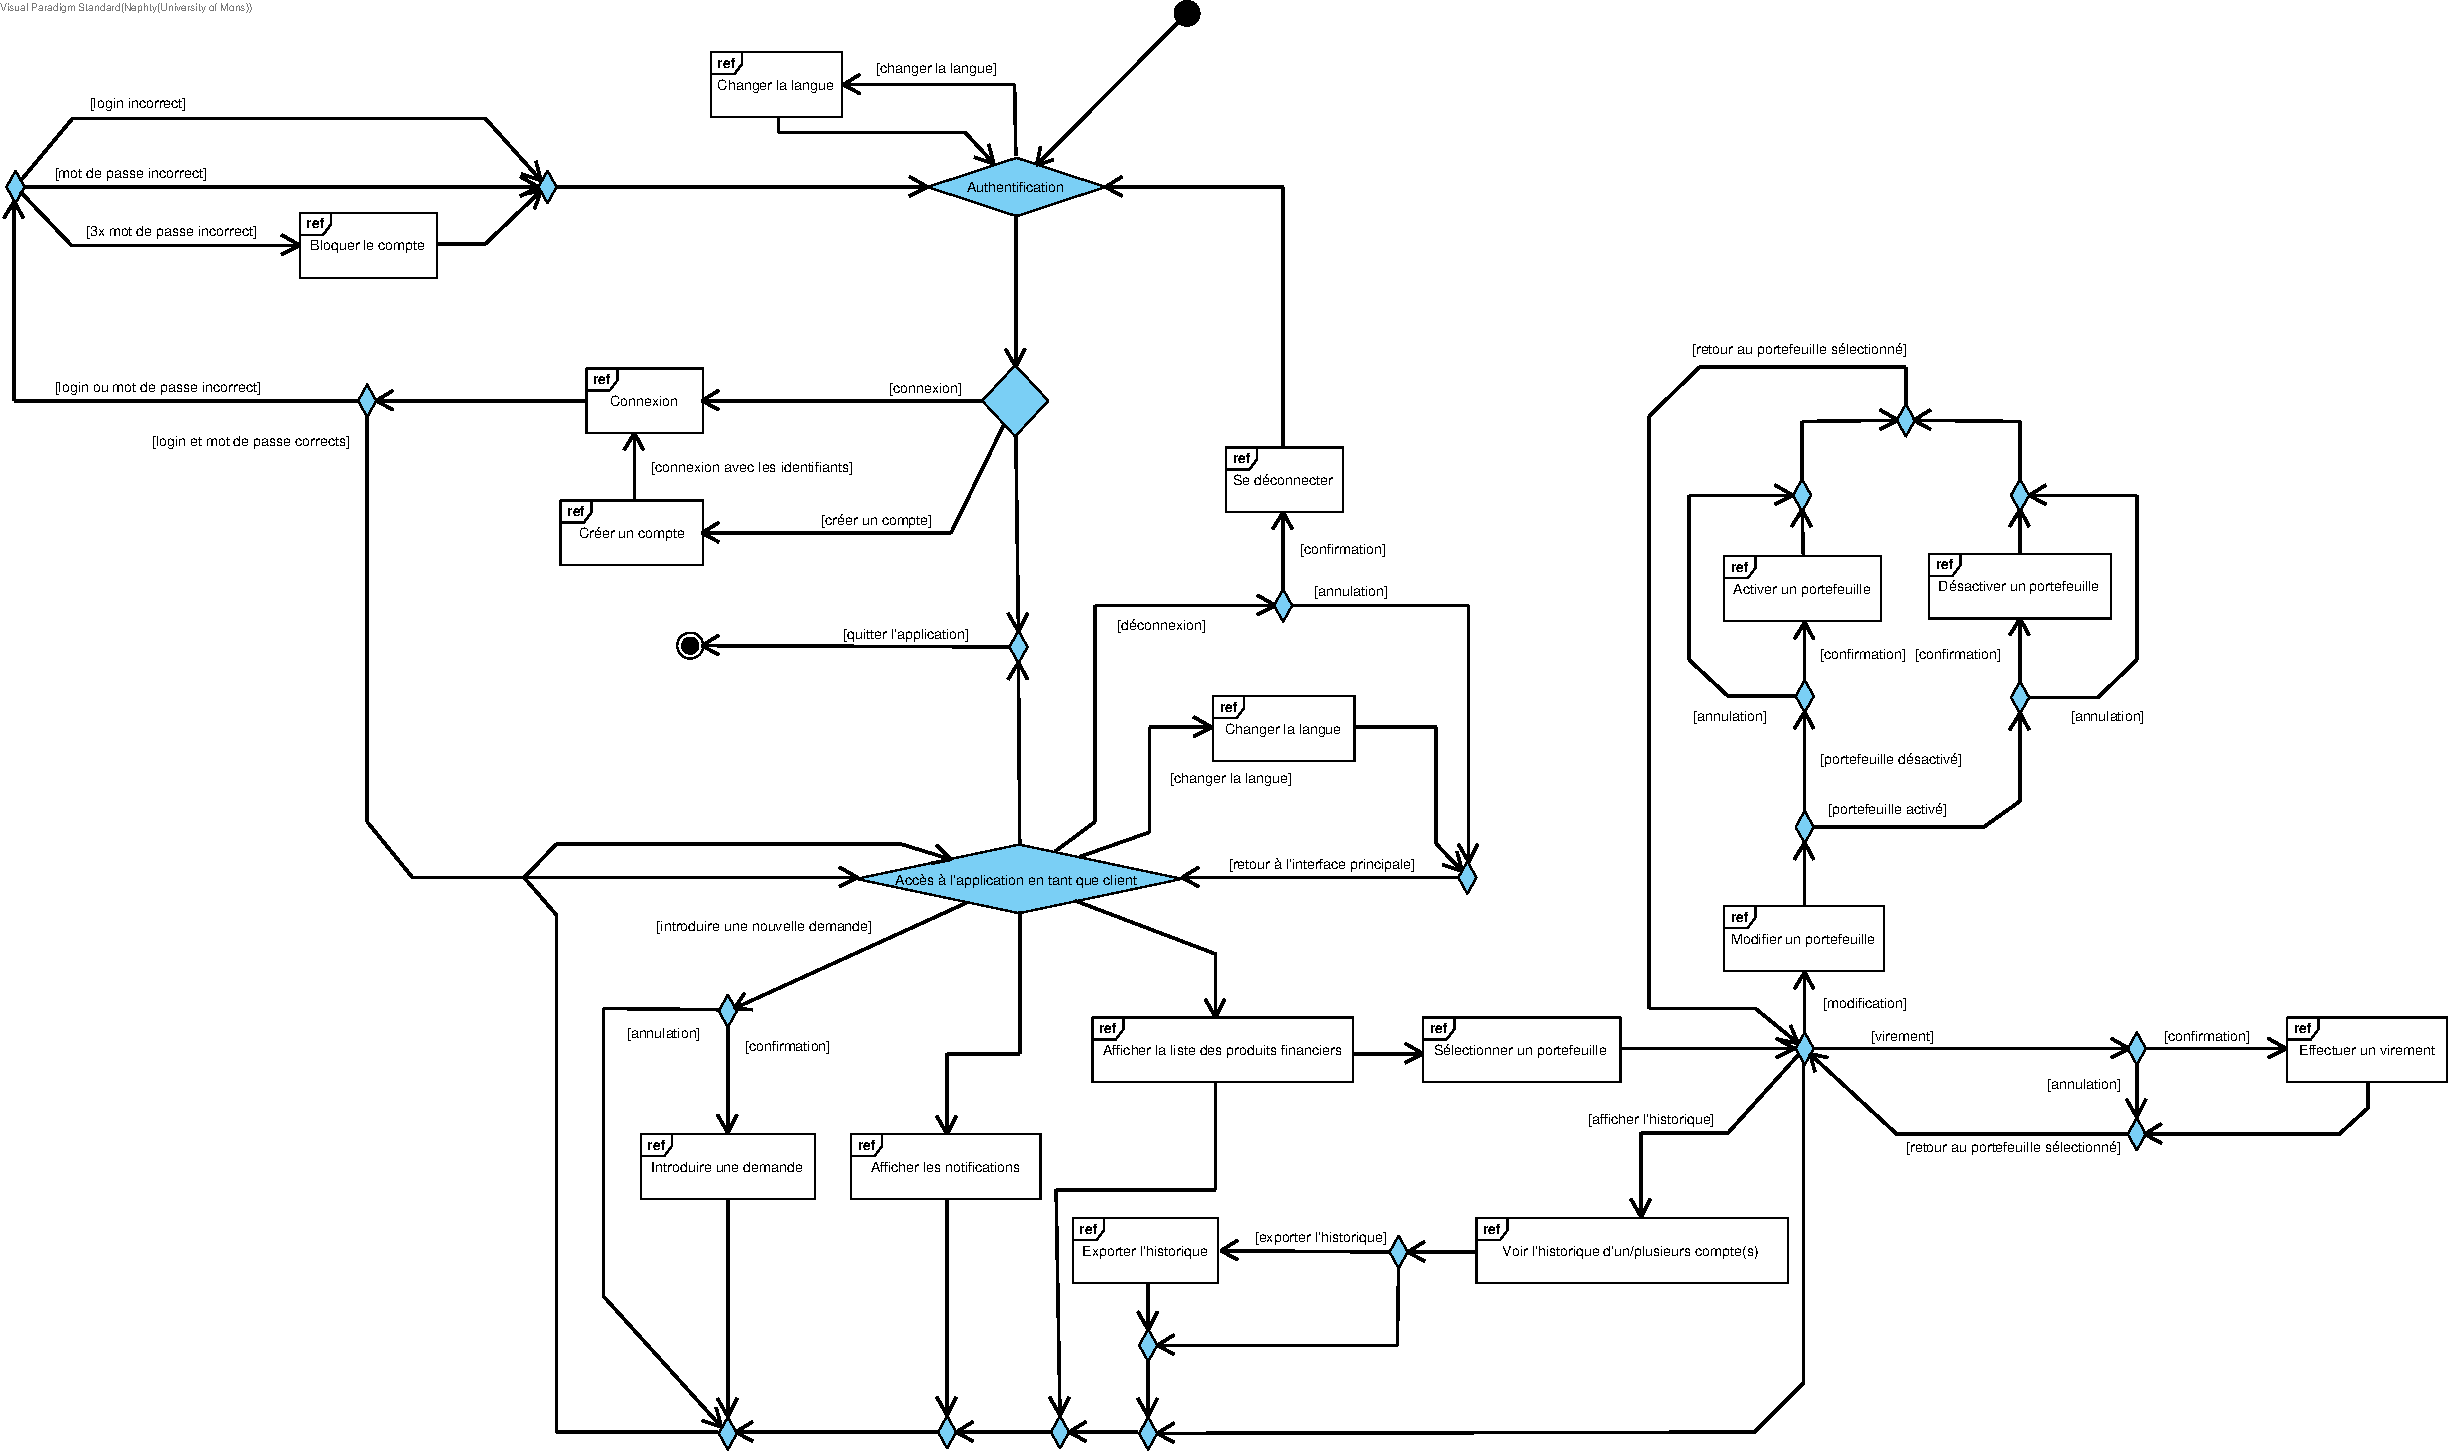
\includegraphics[width=\linewidth]{img/Interaction Overview Client.pdf}
}
\caption{Interaction overview diagram : application client}
\end{figure}

\newpage


\subsection{Class diagram}

\subfile{subfiles/Class Client commun.tex}

\newpage

\subsection{Sequence diagram}

\subfile{subfiles/SequenceDiagramCommunClient.tex}

\newpage

\subsection{Statechart diagram}

\begin{figure}[h!]
\hspace{2.25cm}
\hbox{
	\centering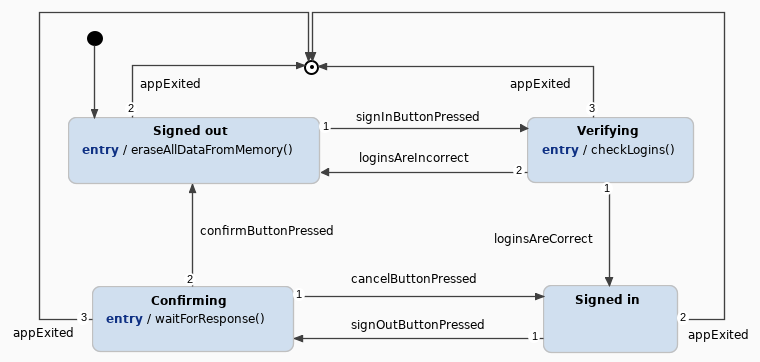
\includegraphics[scale=0.4]{img/statechart.png}
}
\end{figure}

\subfile{subfiles/Statechart.tex}

\newpage



\section{Diagrammes de conception UML : application institution}



\subsection{Use case diagram}

\subfile{subfiles/Use Case Institution.tex}

\begin{figure}[h]
	\centering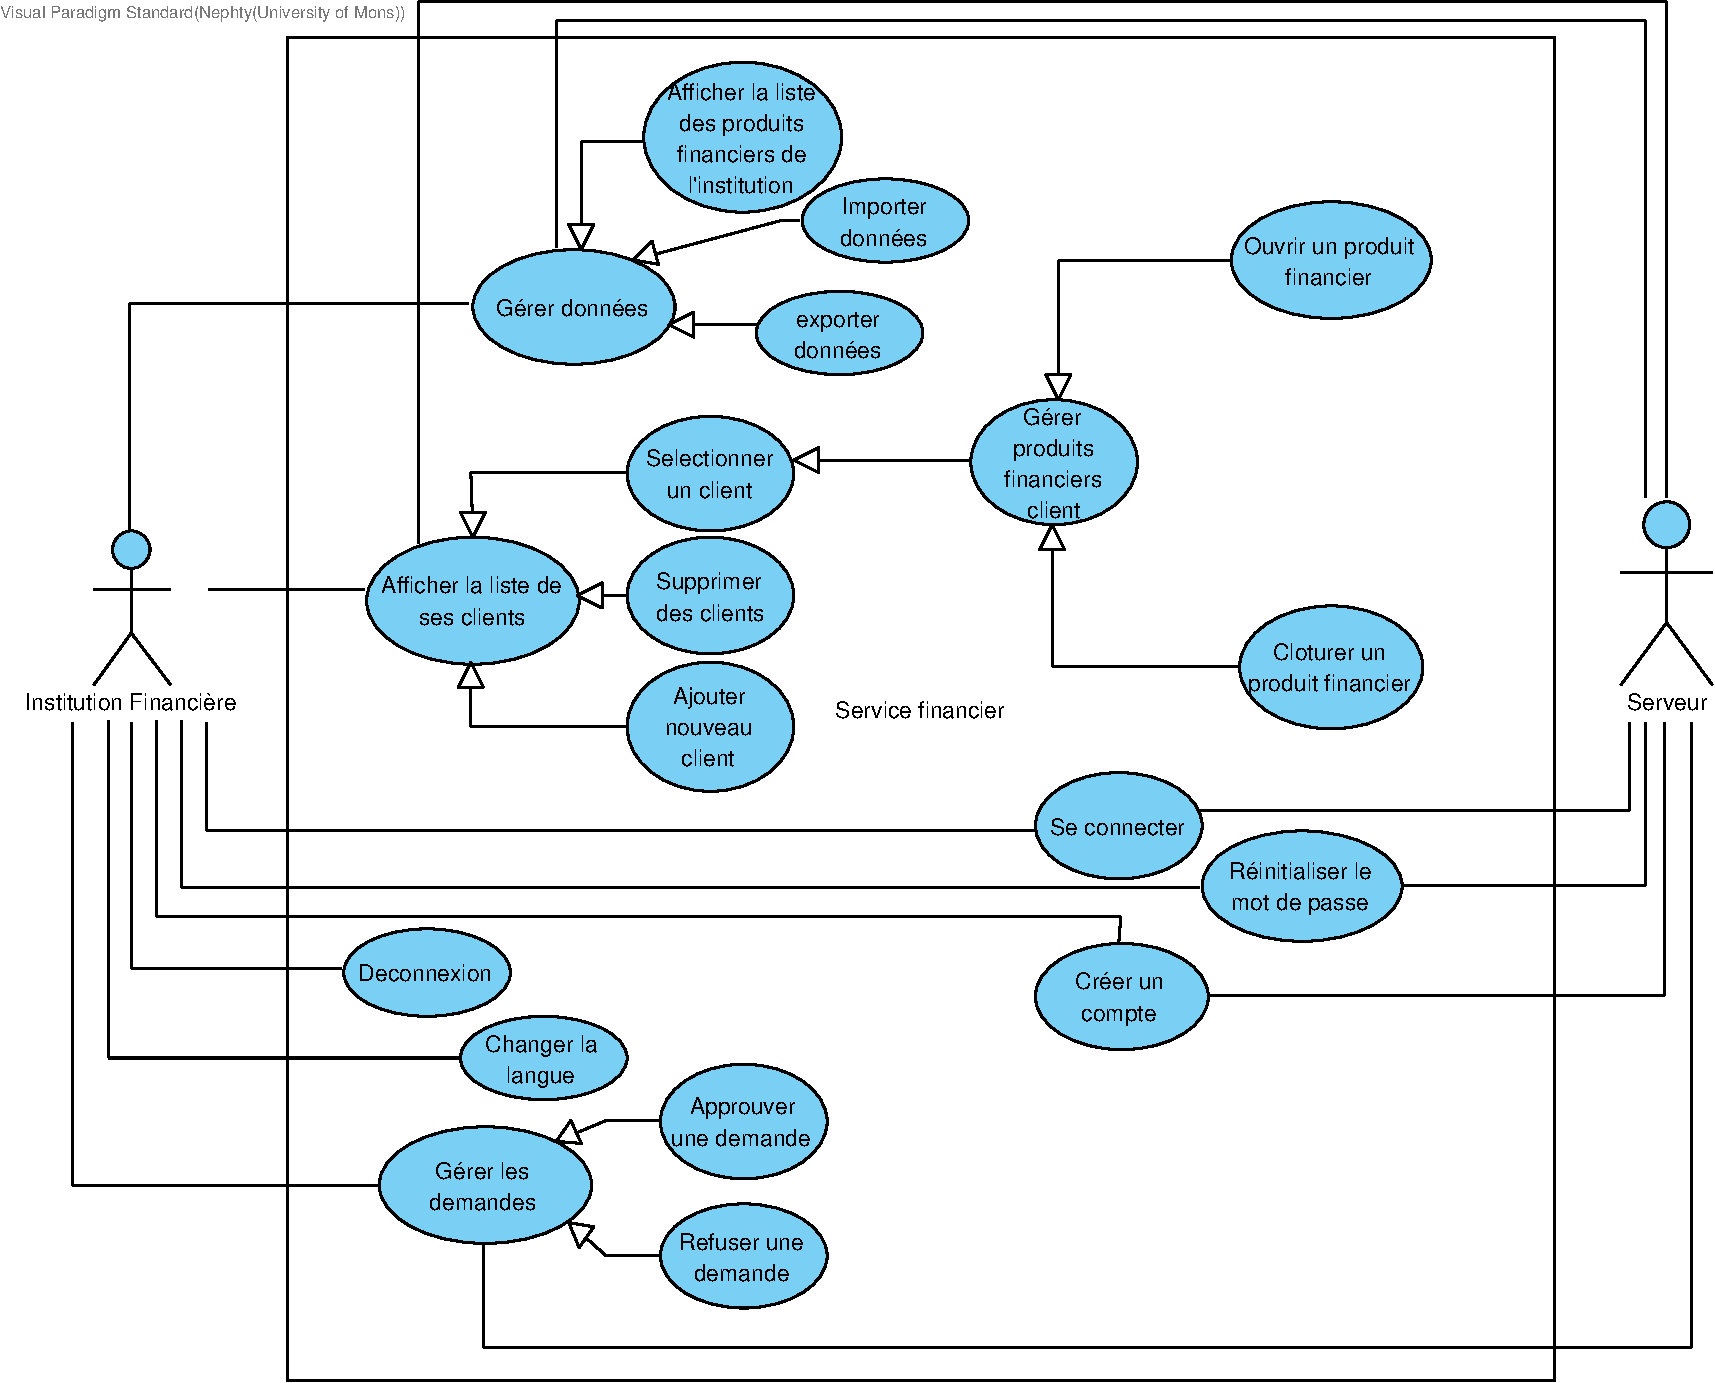
\includegraphics[width=\linewidth]{img/Use Case Institution.pdf}
	\caption{Diagramme de case d'utilisation de l'application pour un service financier.}
\end{figure}

\newpage

\subsection{Interaction overview diagram}

\subfile{subfiles/Interaction Overview Institution.tex}

\vspace{2.5cm}
\begin{figure}[h!]
\hbox{
	\centering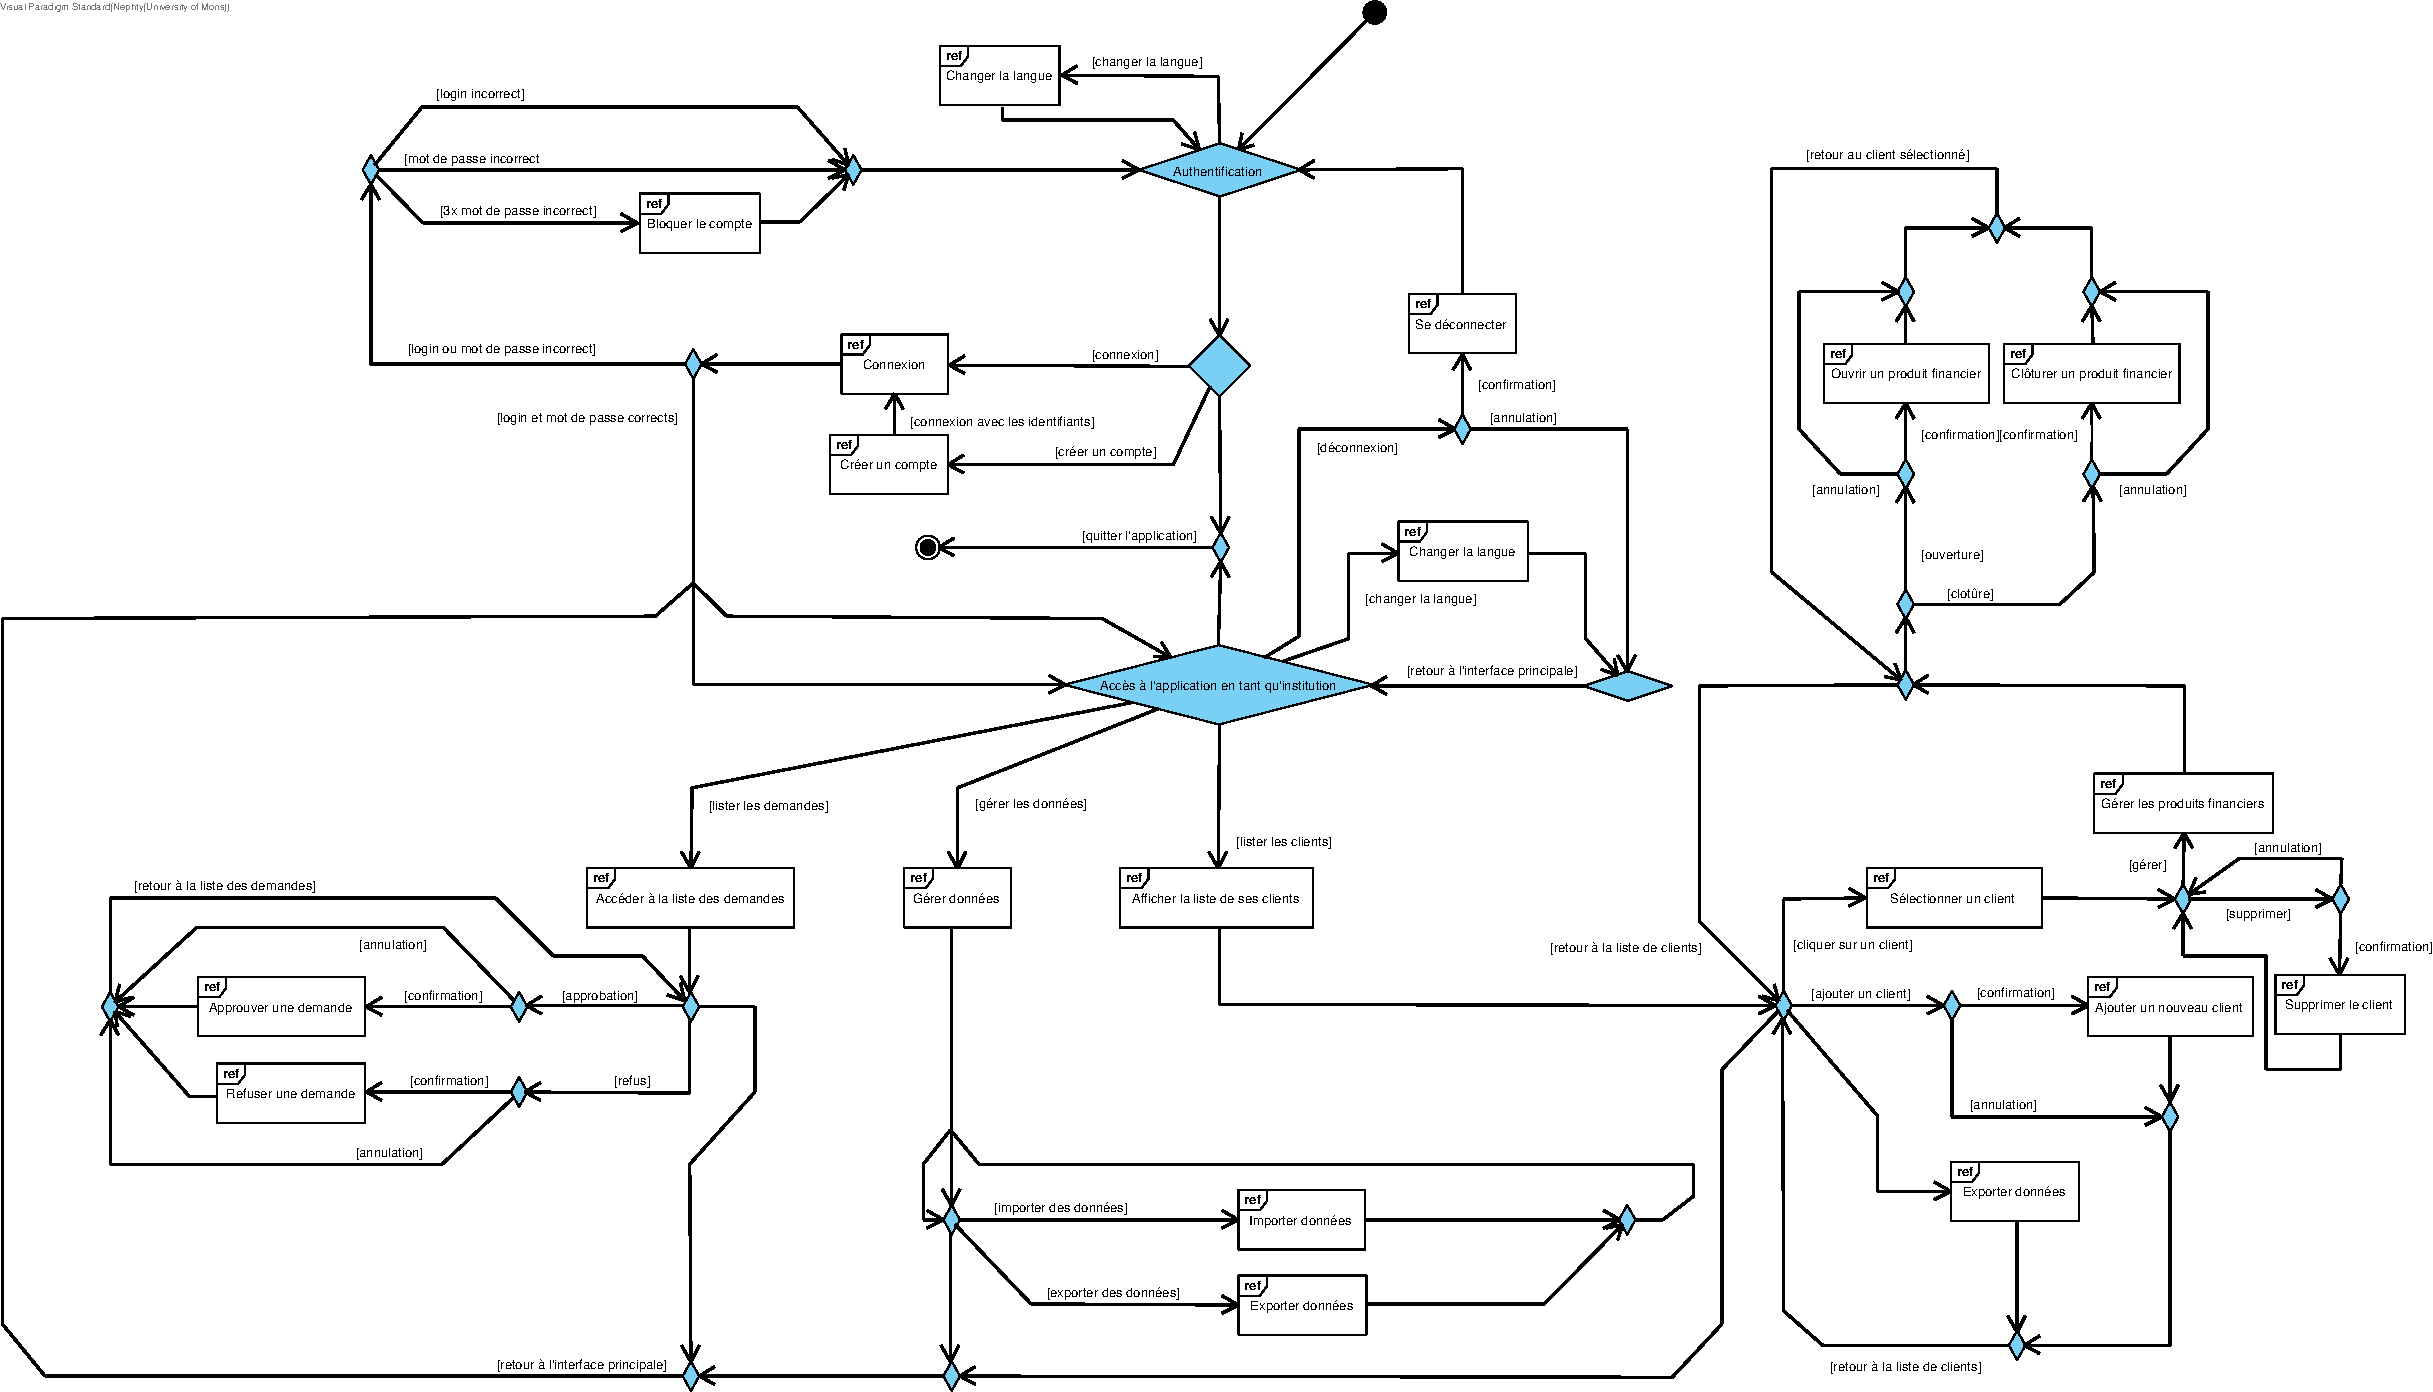
\includegraphics[width=\linewidth]{img/Interaction Overview Institution.pdf}
}
\caption{Interaction overview diagram : application institution}
\end{figure}

\newpage

\subsection{Class diagram}

\subfile{subfiles/Class Banque Commun.tex}

\newpage

\subsection{Sequence diagram}

\subfile{subfiles/sequence-financiere-commun-ltx.tex}
\newpage

\section{Modèle de données}

\begin{figure}[h]
	\centering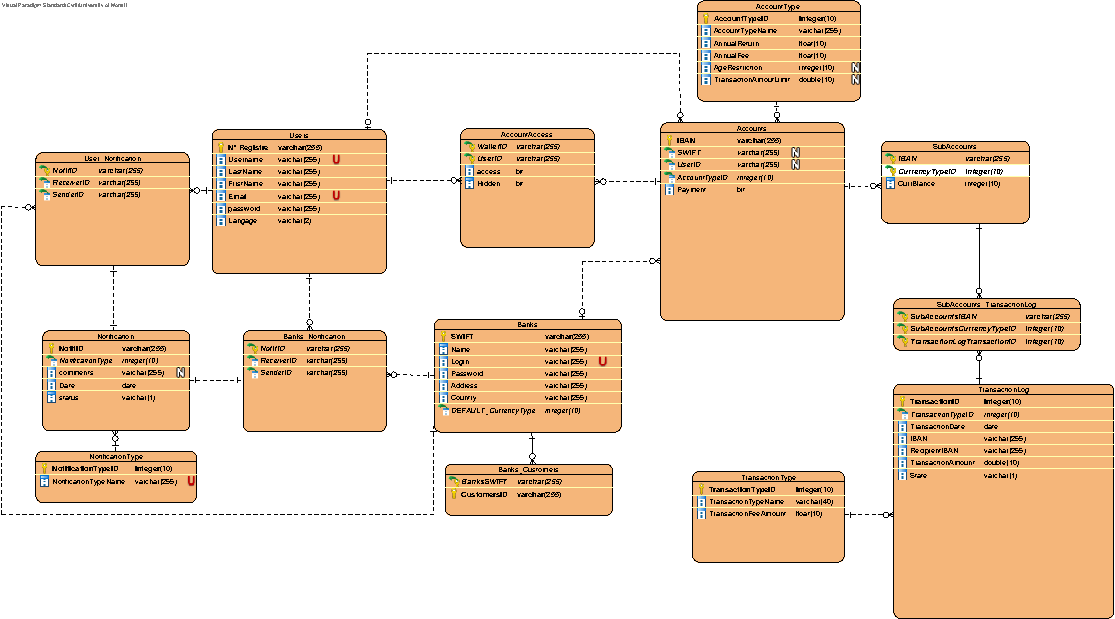
\includegraphics[width=\linewidth]{img/BDD.pdf}
	\caption{Diagramme d'entite relation}
\end{figure}
\subfile{subfiles/BDD.tex}

\newpage


\section{Design du REST API}

\begin{figure}[h]
	\centering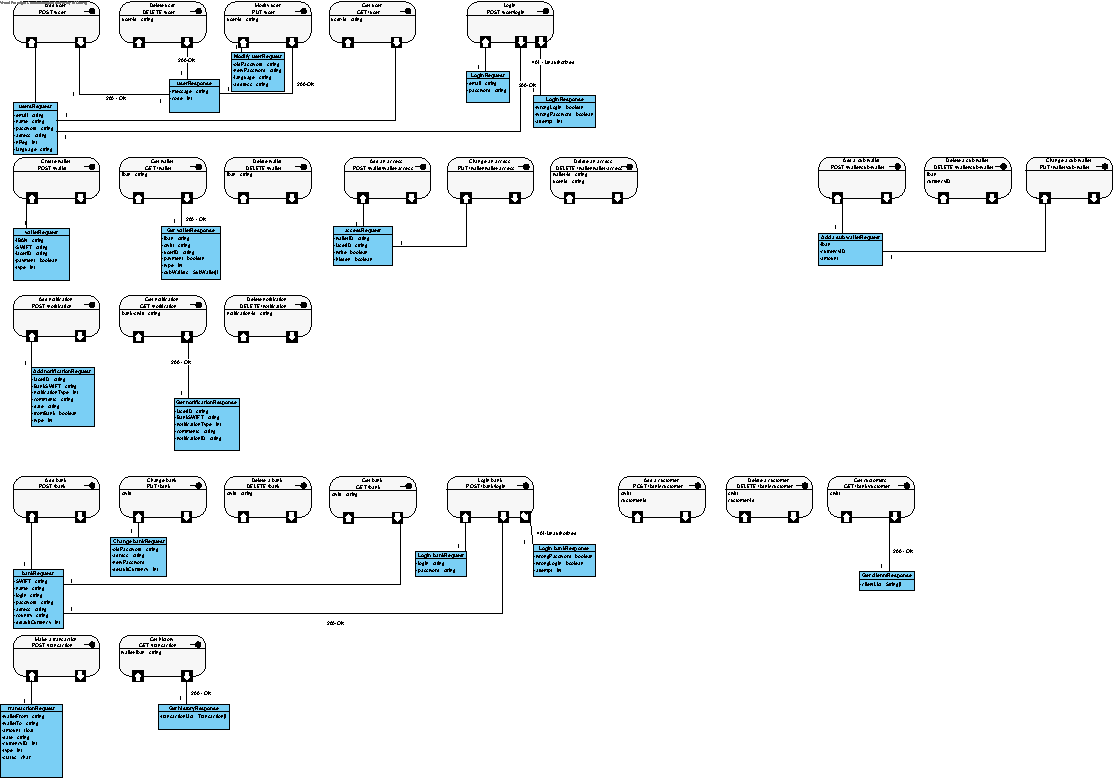
\includegraphics[width=\linewidth]{img/rest-api-commun.pdf}
	\caption{Diagramme de l'API}
\end{figure}

\subfile{subfiles/rest-api-commun-ltx.tex}


\newpage


\section{Maquette de l'interface utilisateur : application client}

\subfile{subfiles/UI Client.tex}

\vspace*{\fill}

\paragraph{Illustration du diagramme} Par souci de clareté, ce diagramme est disponible en annexe du rapport.

\newpage



\section{Maquette de l'interface utilisateur : application institution}

\subfile{subfiles/UI Institution.tex}

\vspace*{\fill}

\paragraph{Illustration du diagramme} Par souci de clareté, ce diagramme est disponible en annexe du rapport.

\newpage





\chapter{Extension A : Gestion de cartes - Augustin \textsc{Houba}}



\newpage


\section{Diagrammes de conception UML : application client}

\subsection{Use case diagram}
\begin{figure}[h]
	\centering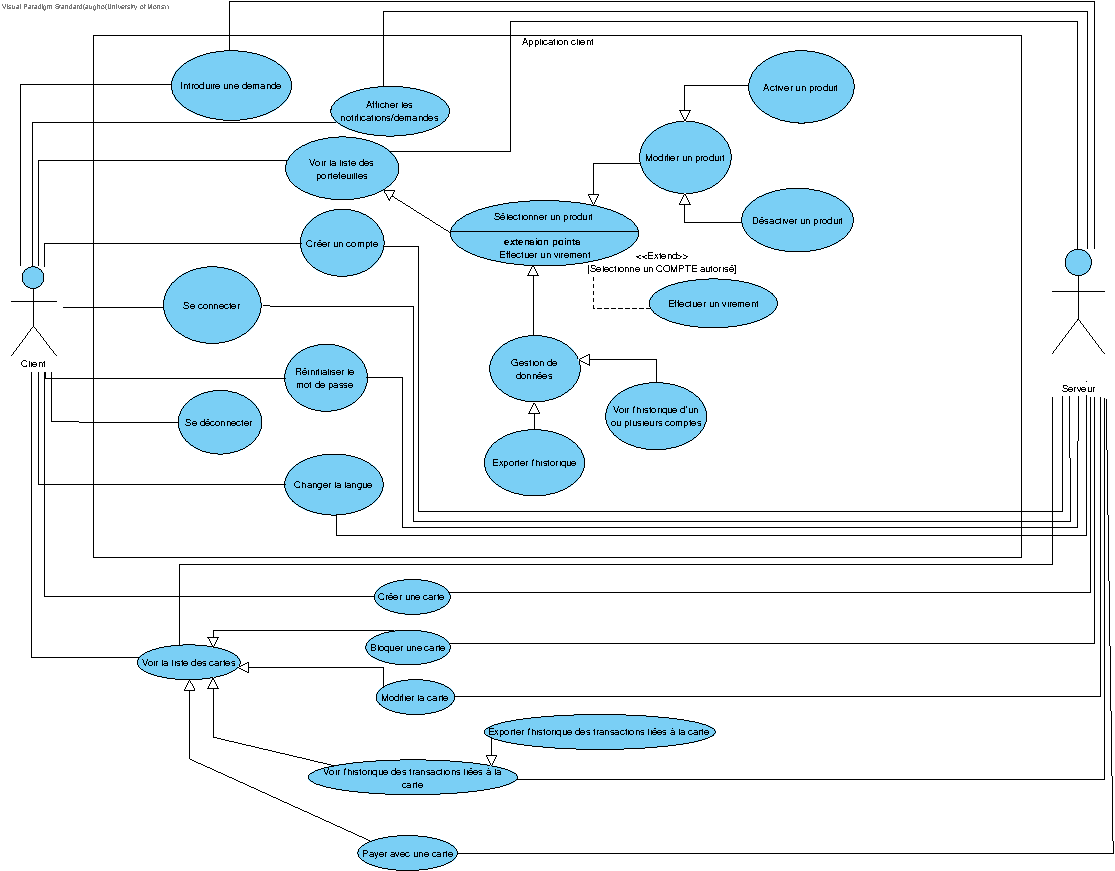
\includegraphics[width=\linewidth]{img/use-case-Extension-1.pdf}
	\caption{Use case diagram - Extension 1}
\end{figure}

\subfile{subfiles/use-case-Extension-1-ltx.tex}


\newpage

\subsection{Interaction overview diagram}

\begin{figure}[h!]
	\centering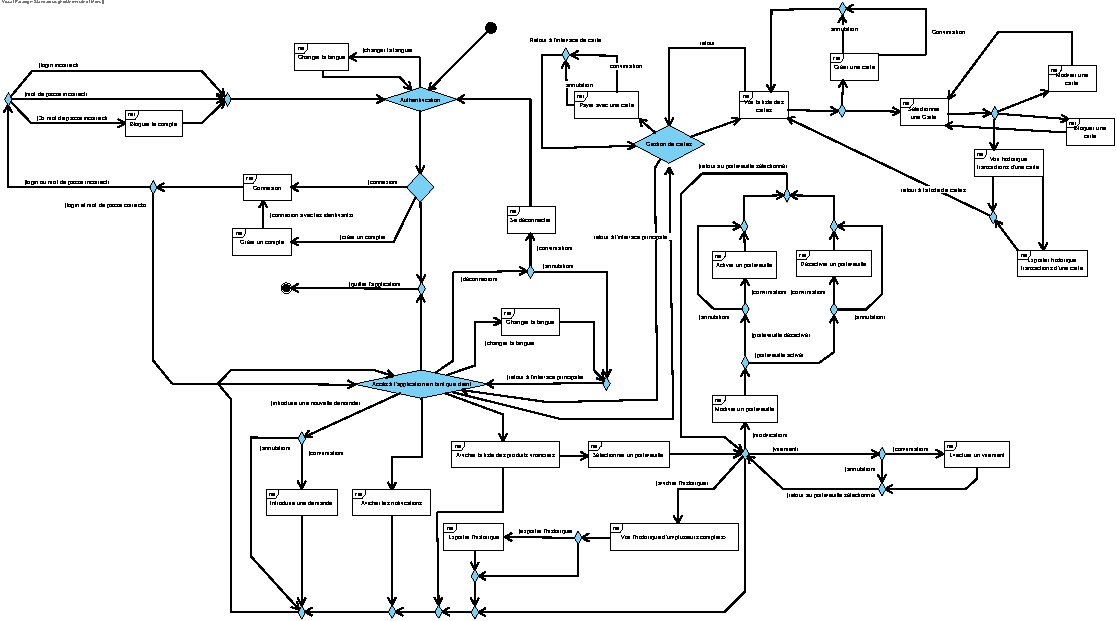
\includegraphics[width=\linewidth]{img/iov-client-Extension-1.pdf}
	\caption{Interaction overview diagram - Extension 1}
\end{figure}

\subfile{subfiles/iov-client-Extension-1-ltx.tex}

\newpage

\subsection{Class diagram}

\begin{figure}[h!]
	\centering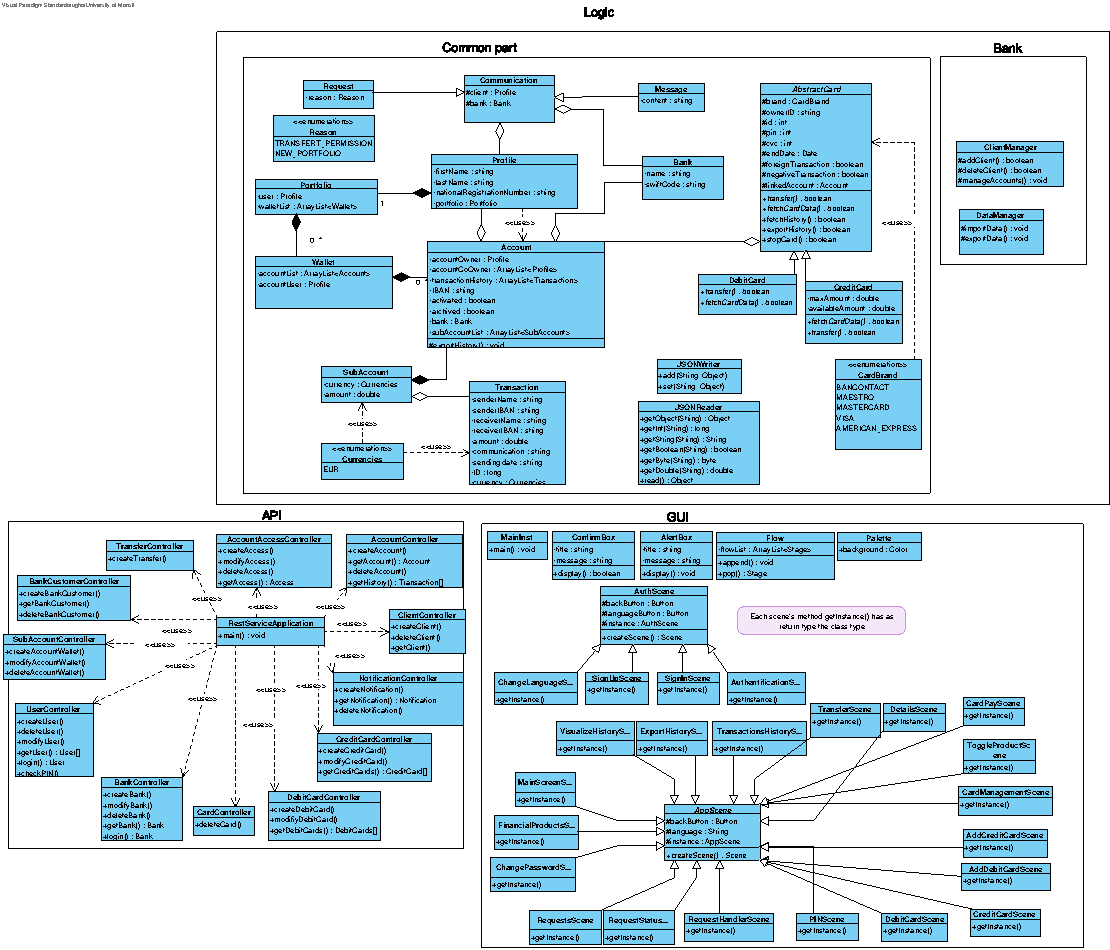
\includegraphics[width=\linewidth]{img/class-Extension-1.pdf}
	\caption{Diagramme de classes - Extension 1}
\end{figure}

\subfile{subfiles/class-Extension-1-ltx.tex}

\newpage

\subsection{Sequence diagram}

\subfile{subfiles/sequence-client-Extension-1-ltx.tex}

\newpage



\section{Diagrammes de conception UML : application institution}



\subsection{Use case diagram}

Il n'y a pas de changement par rapport à l'application de base


\subsection{Interaction overview diagram}

Il n'y a pas de changement par rapport à l'application de base

\subsection{Class diagram}

Il n'y a pas de changement par rapport à l'application de base

\subsection{Sequence diagram}

Il n'y a pas de changement par rapport à l'application de base

\newpage

\section{Maquette de l'interface utilisateur: application client}

\begin{figure}[h!]
	\centering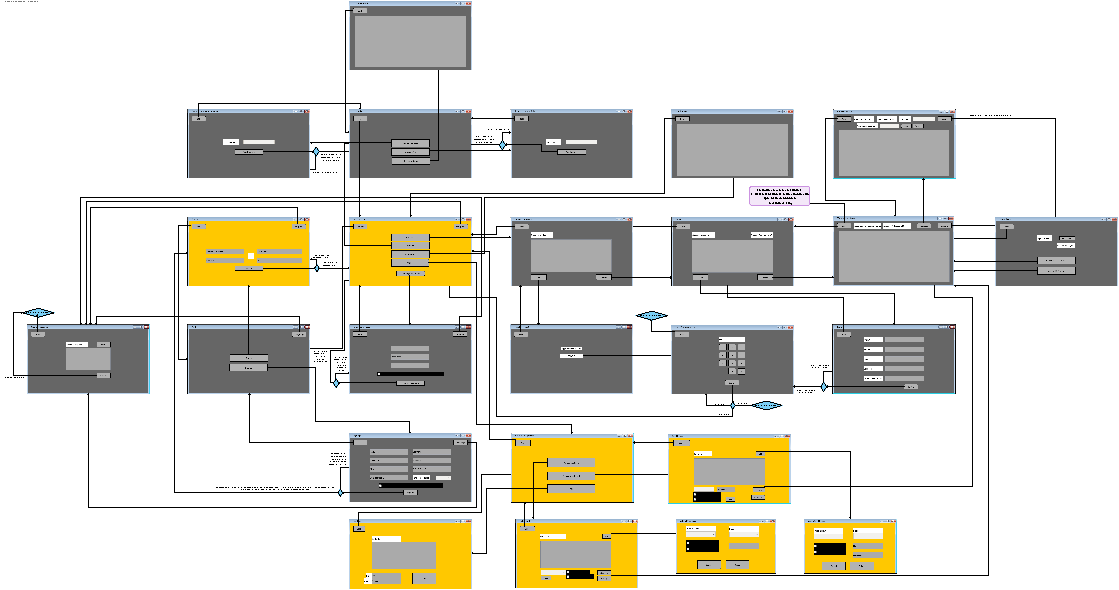
\includegraphics[width=\linewidth]{img/UI-client-Extension-1.pdf}
	\caption{Maquette de l'interface utilisateur: application client - Extension 1}
\end{figure}

\subfile{subfiles/UI-client-Extension-1-ltx.tex}

\newpage
\section{Maquette de l'interface utilisateur: application institution}

\begin{figure}[h!]
	\centering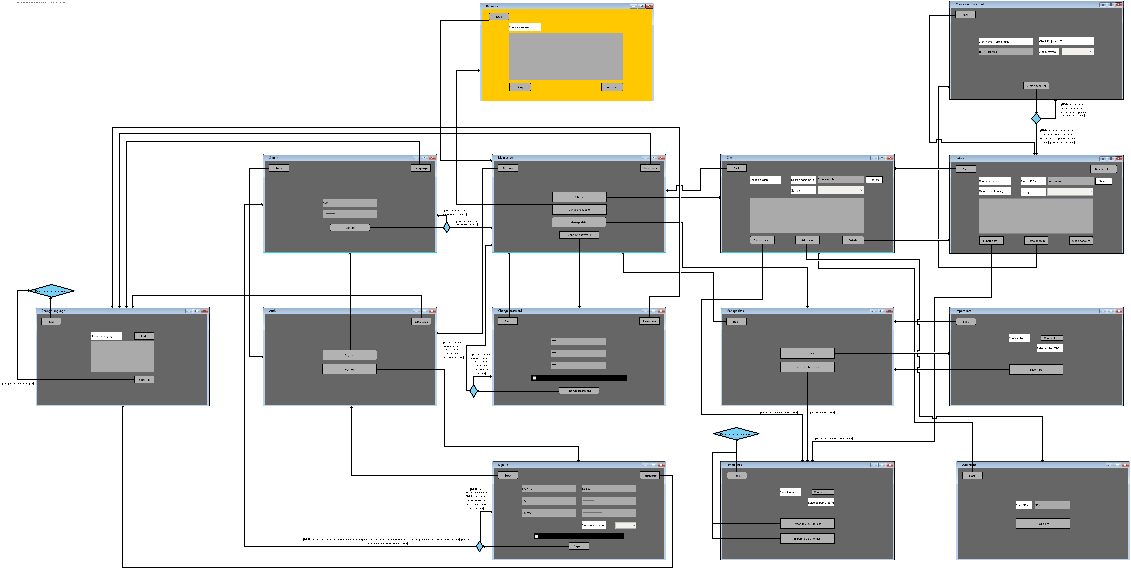
\includegraphics[width=\linewidth]{img/ui-institution-Extension-1.pdf}
	\caption{Maquette de l'interface utilisateur: application institution - Extension 1}
\end{figure}

\subfile{subfiles/ui-institution-Extension-1-ltx.tex}
\newpage
\section{Design du REST API}

\begin{figure}[h!]
	\centering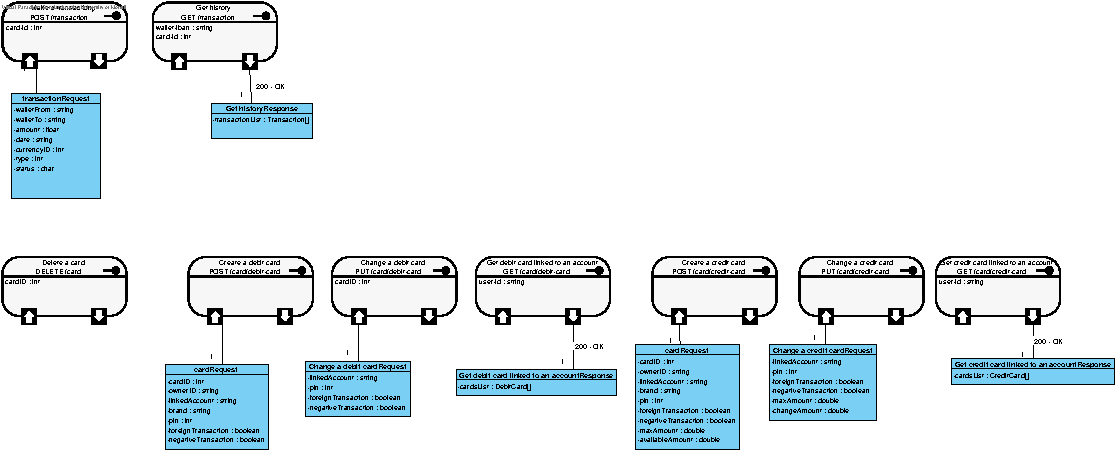
\includegraphics[width=\linewidth]{img/rest-api-Extension-1.pdf}
	\caption{Maquette de l'interface utilisateur: application client - Extension 1}
\end{figure}

\subfile{subfiles/rest-api-Extension-1-ltx.tex}

\newpage

\section{Modèle de données}

\begin{figure}[h!]
	\centering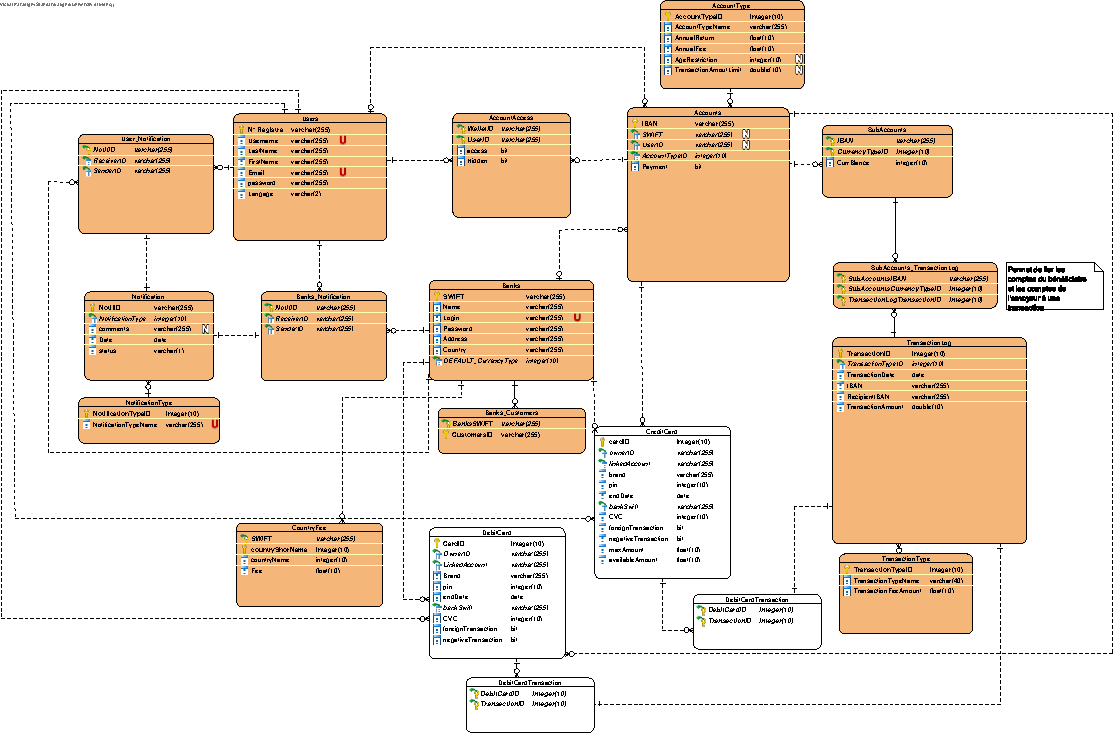
\includegraphics[width=\linewidth]{img/bdd-extension-1.pdf}
	\caption{Modèle de base de données - Extension 1}
\end{figure}

\subfile{subfiles/bdd-extension-1.tex}

\newpage




\chapter{Extension B : Gestion de devises et virements internationaux - Cyril \textsc{Moreau}}



\newpage



\section{Diagrammes de conception UML : application client}



\subsection{Use case diagram}

\begin{figure}[h]
	\centering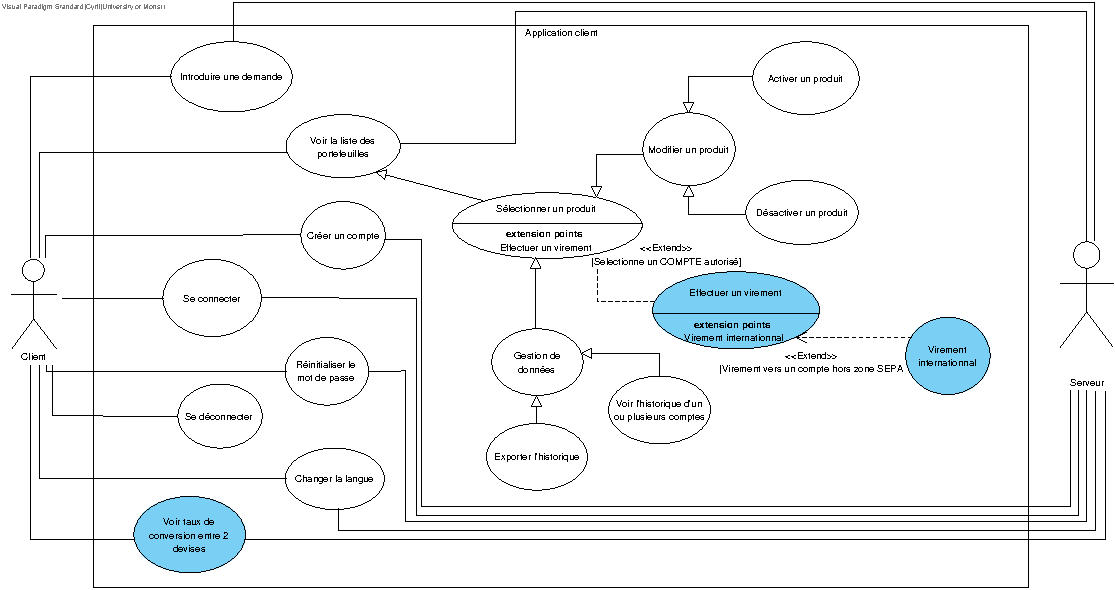
\includegraphics[width=\linewidth]{img/Use Case Client - Extension 2.pdf}
	\caption{Diagramme de case d'utilisation de l'application client de l'extension 2.}
\end{figure}
\subfile{subfiles/Use Case Client - Extension 2.tex}
\newpage

\subsection{Interaction overview diagram}

\begin{figure}[h]
	\centering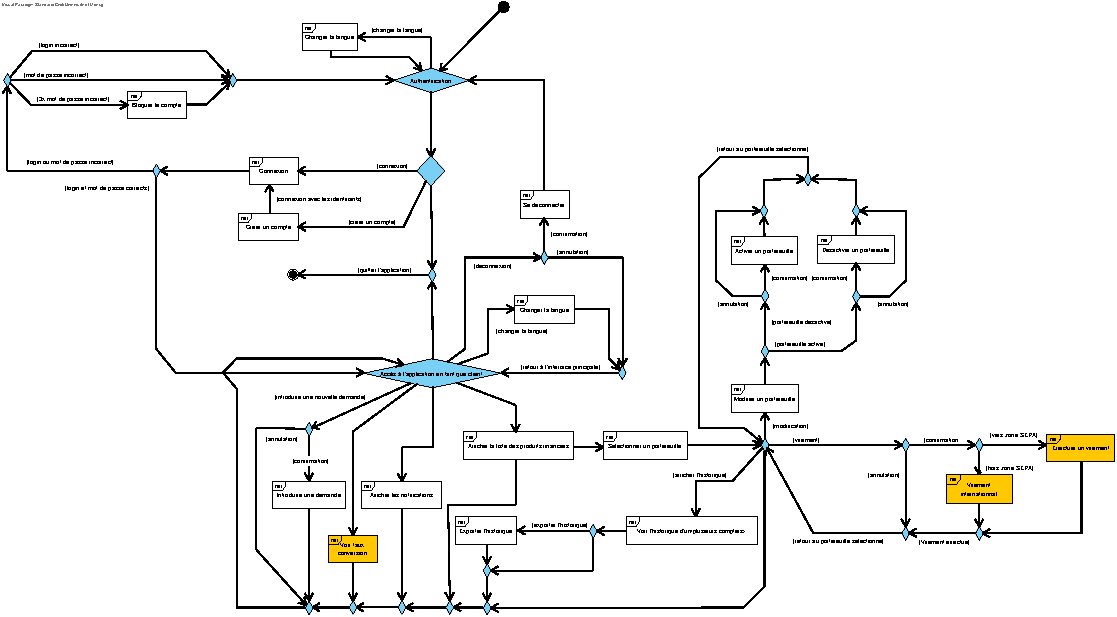
\includegraphics[width=\linewidth]{img/Interaction Overview Client - Extension 2.pdf}
	\caption{Interaction overview diagram de l'application client de l'extension 2.}
\end{figure}
\subfile{subfiles/Interaction Overview Client - Extension 2.tex}

\newpage

\subsection{Class diagram}

\begin{figure}[h!]
	\hbox{
		\centering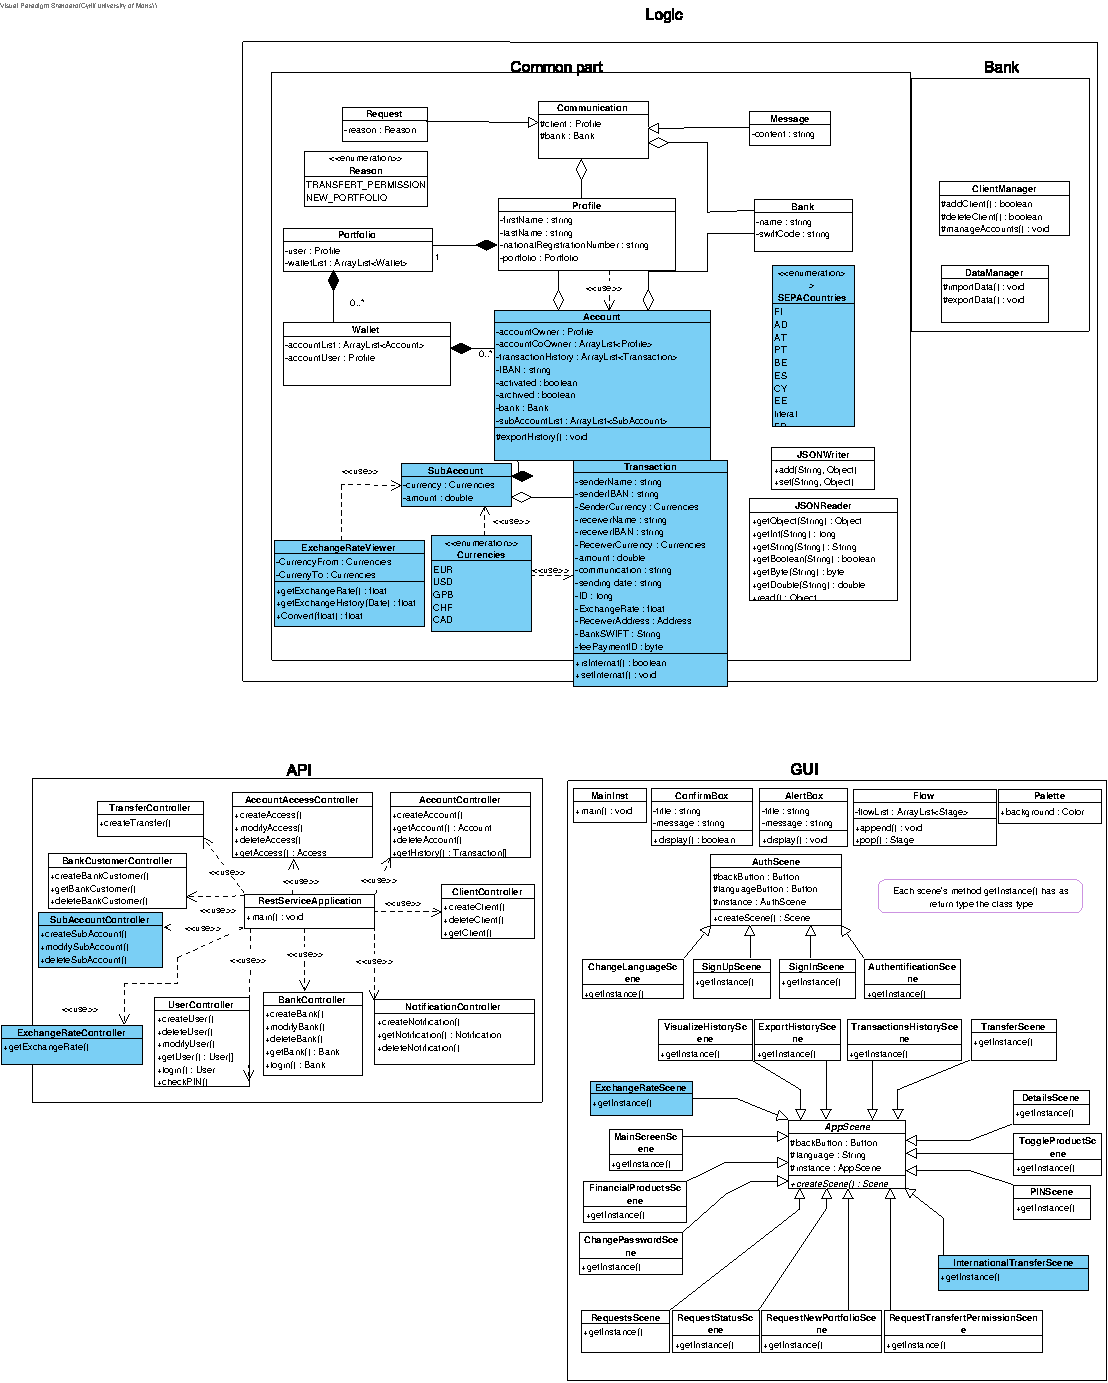
\includegraphics[scale=0.69]{img/Class Diagram Client - Extension 2.pdf}
	}
	\caption{Diagramme de classe de l'application client de l'extension 2}
\end{figure}
\newpage
\subfile{subfiles/Class Client - Extension 2.tex}
\newpage

\subsection{Sequence diagram}

\begin{figure}[h!]
	\hbox{
		\centering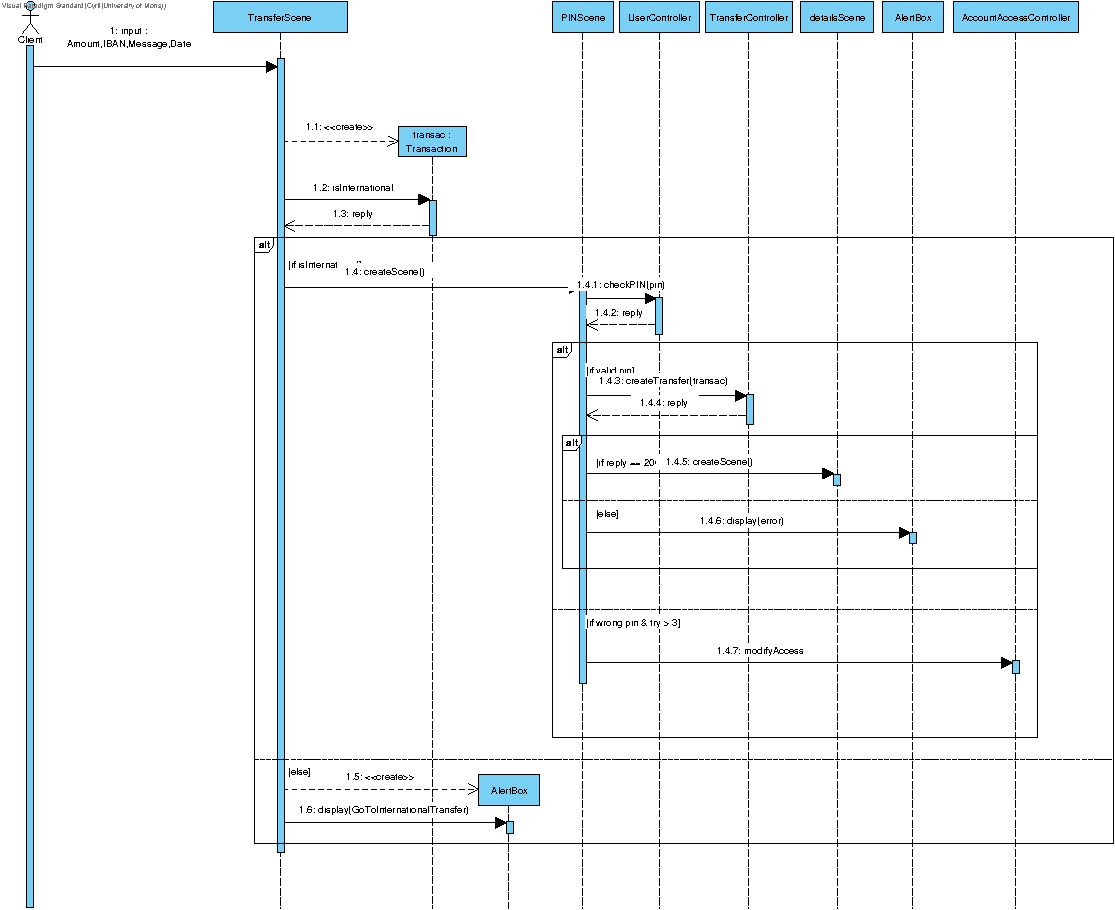
\includegraphics[scale=0.69]{img/Sequence 1 - Extension 2.pdf}
	}
	\caption{Effectuer un virement}
	\end{figure}
\subfile{subfiles/Sequence 1 - Extension 2.tex}
\newpage

\begin{figure}[h!]
	\hbox{
		\centering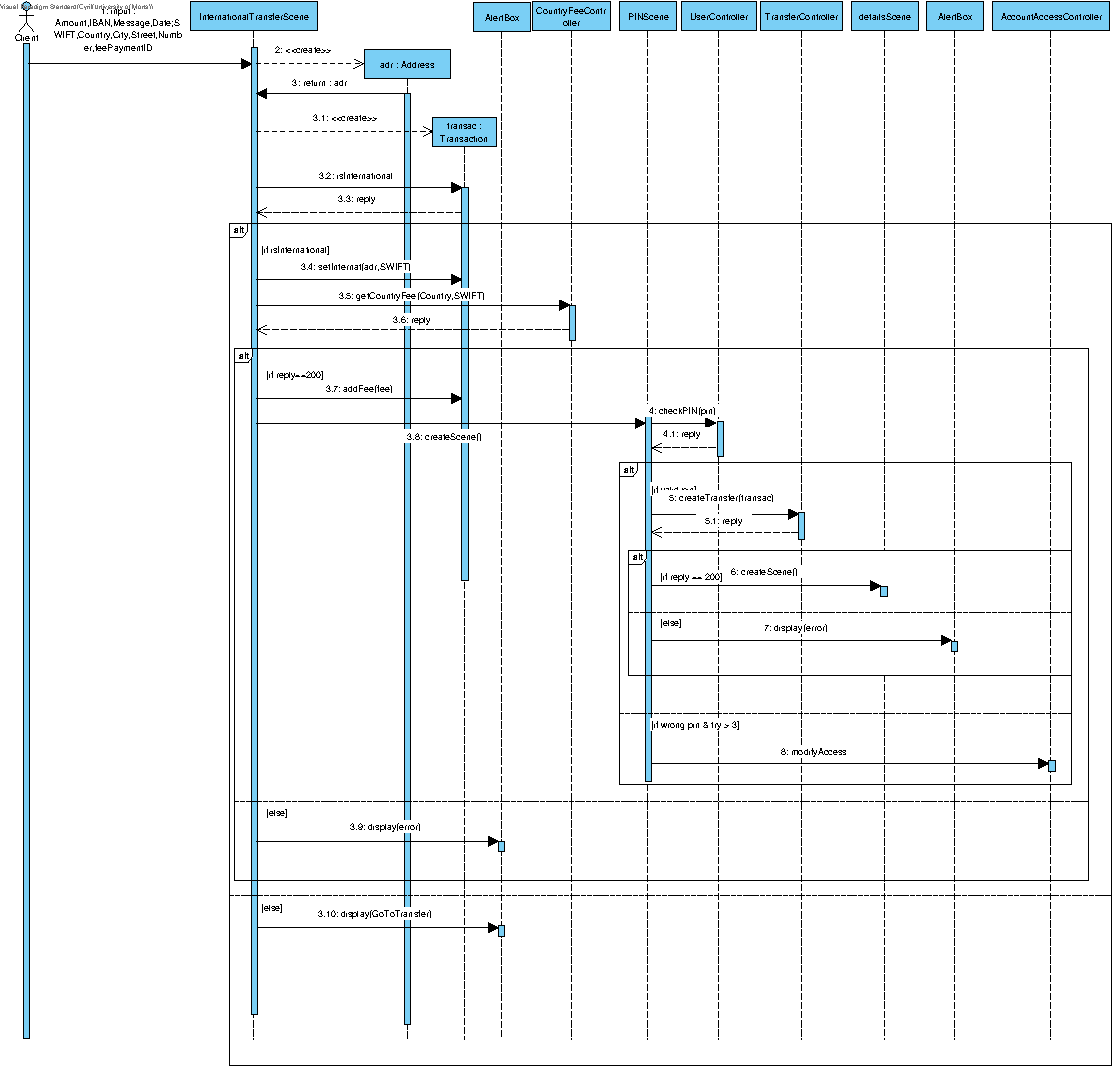
\includegraphics[scale=0.8]{img/Sequence 2 - Extension 2.pdf}
	}
	\caption{Virement international}
	\end{figure}
\subfile{subfiles/Sequence 2 - Extension 2.tex}
\newpage

\begin{figure}[h!]
	\hbox{
		\centering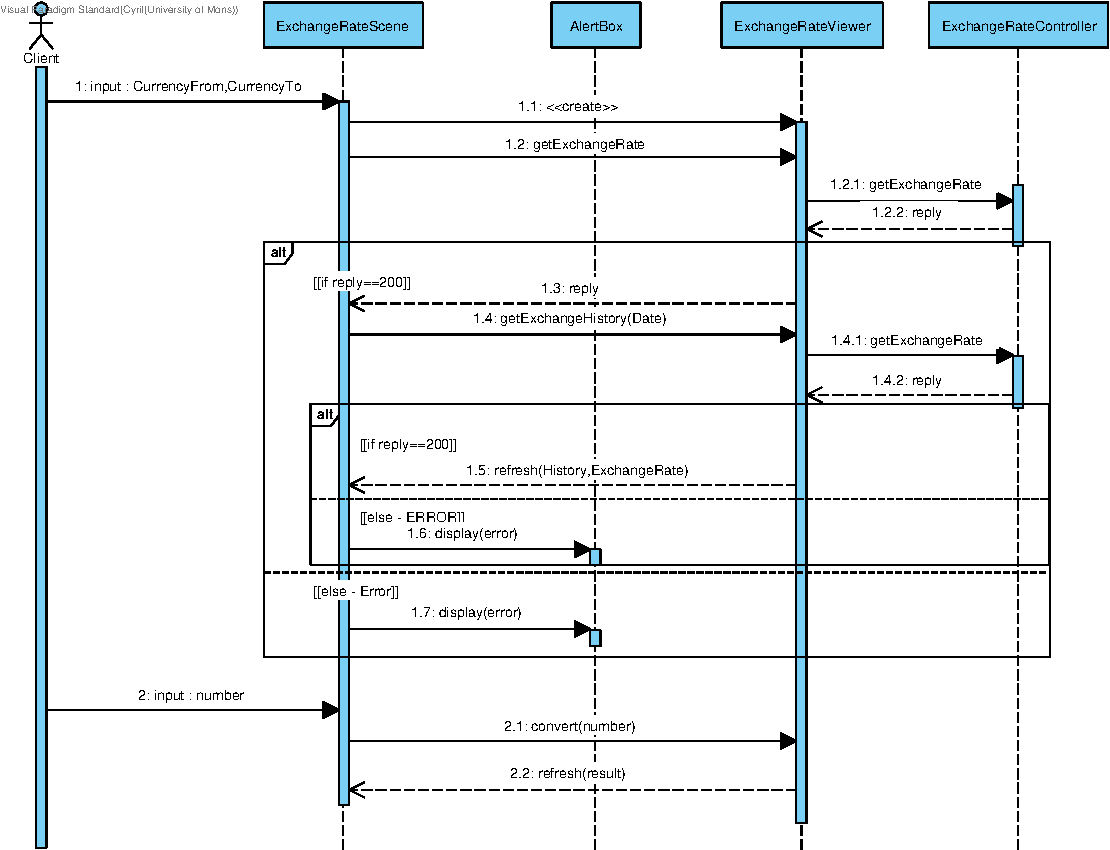
\includegraphics[width=\linewidth]{img/Sequence 3 - Extension 2.pdf}
	}
	\caption{Voir taux conversion}
\end{figure}
\subfile{subfiles/Sequence 3 - Extension 2.tex}
\newpage



\section{Diagrammes de conception UML : application institution}



\subsection{Use case diagram}

\begin{figure}[h]
	\centering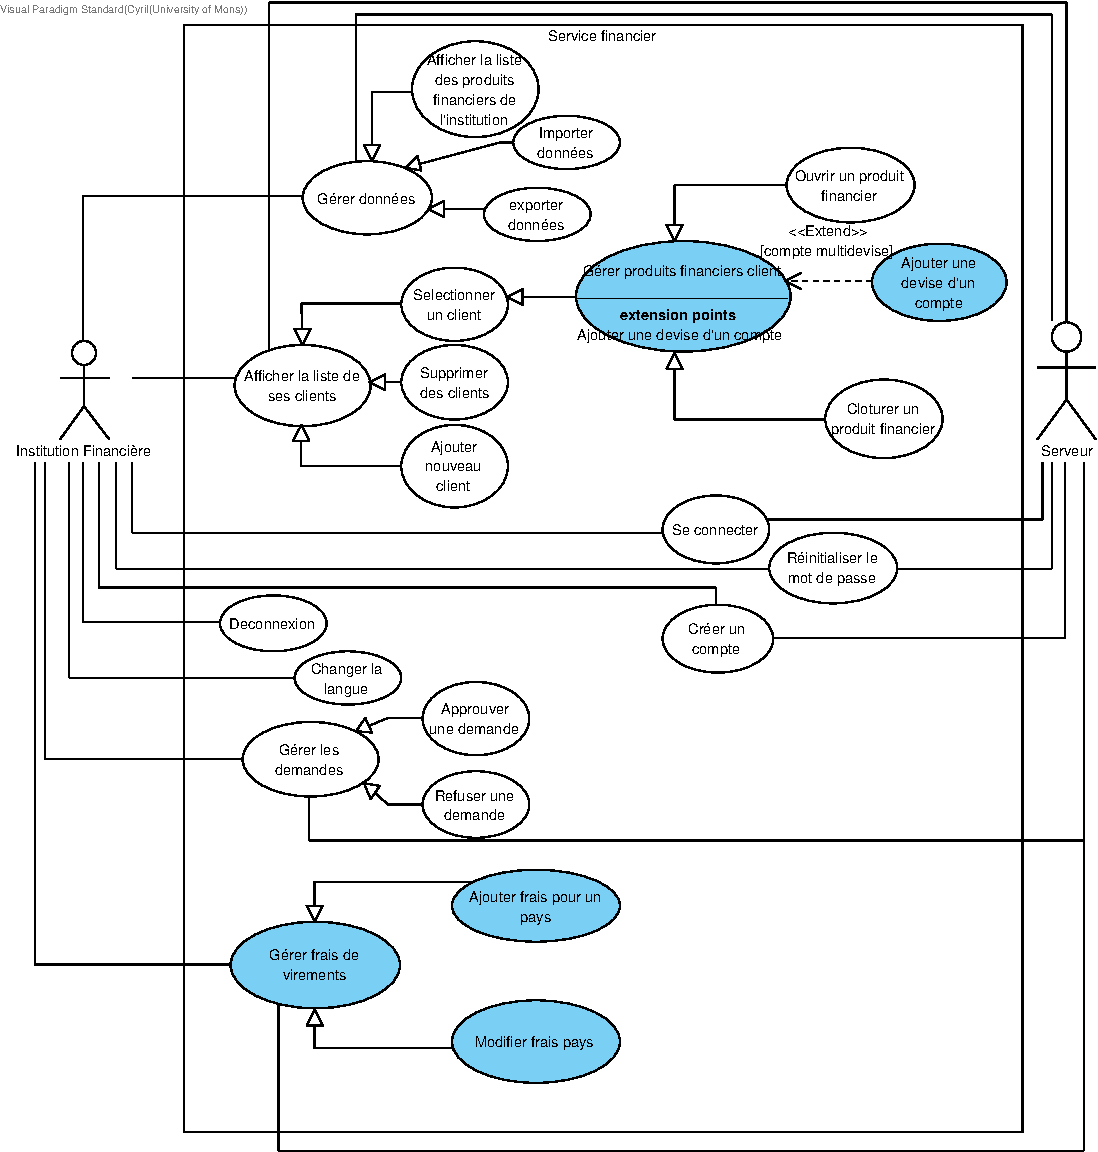
\includegraphics[scale=0.45]{img/Use Case Institution - Extension 2.pdf}
	\caption{Diagramme de case d'utilisation de l'application service financier de l'extension 2.}
\end{figure}
\subfile{subfiles/Use Case Institution - Extension 2.tex}

\newpage

\subsection{Interaction overview diagram}

\begin{figure}[h]
	\centering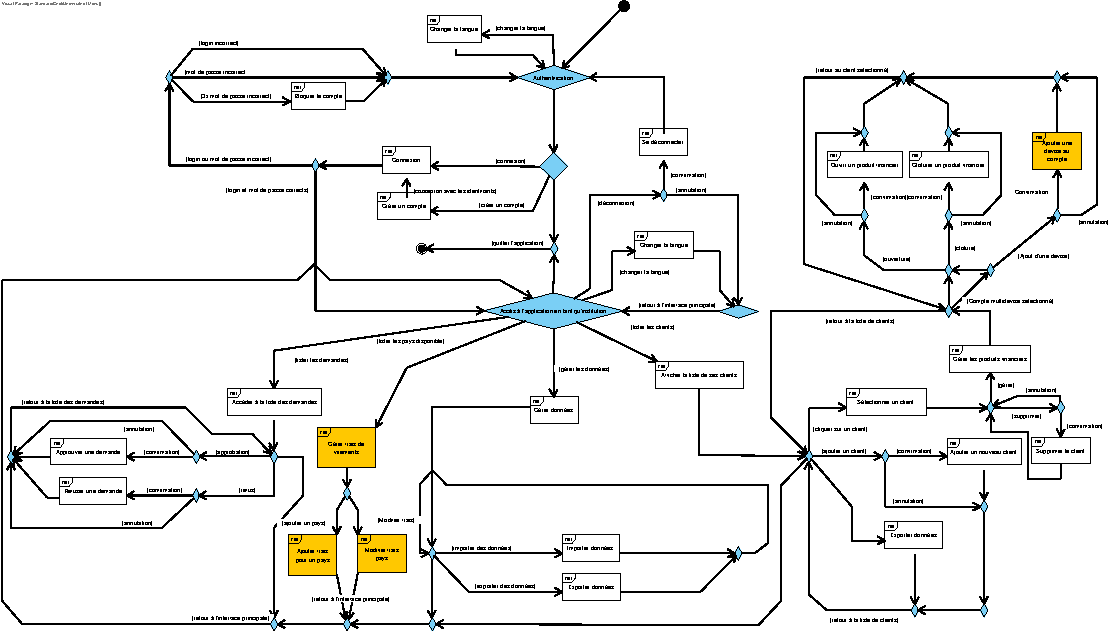
\includegraphics[width=\linewidth]{img/Interaction Overview Institution - Extension 2.pdf}
	\caption{Interaction overview diagram de l'application service financier de l'extension 2.}
\end{figure}
\subfile{subfiles/Interaction Overview Institution - Extension 2.tex}

\newpage

\subsection{Class diagram}

\begin{figure}[h!]
	\hbox{
		\centering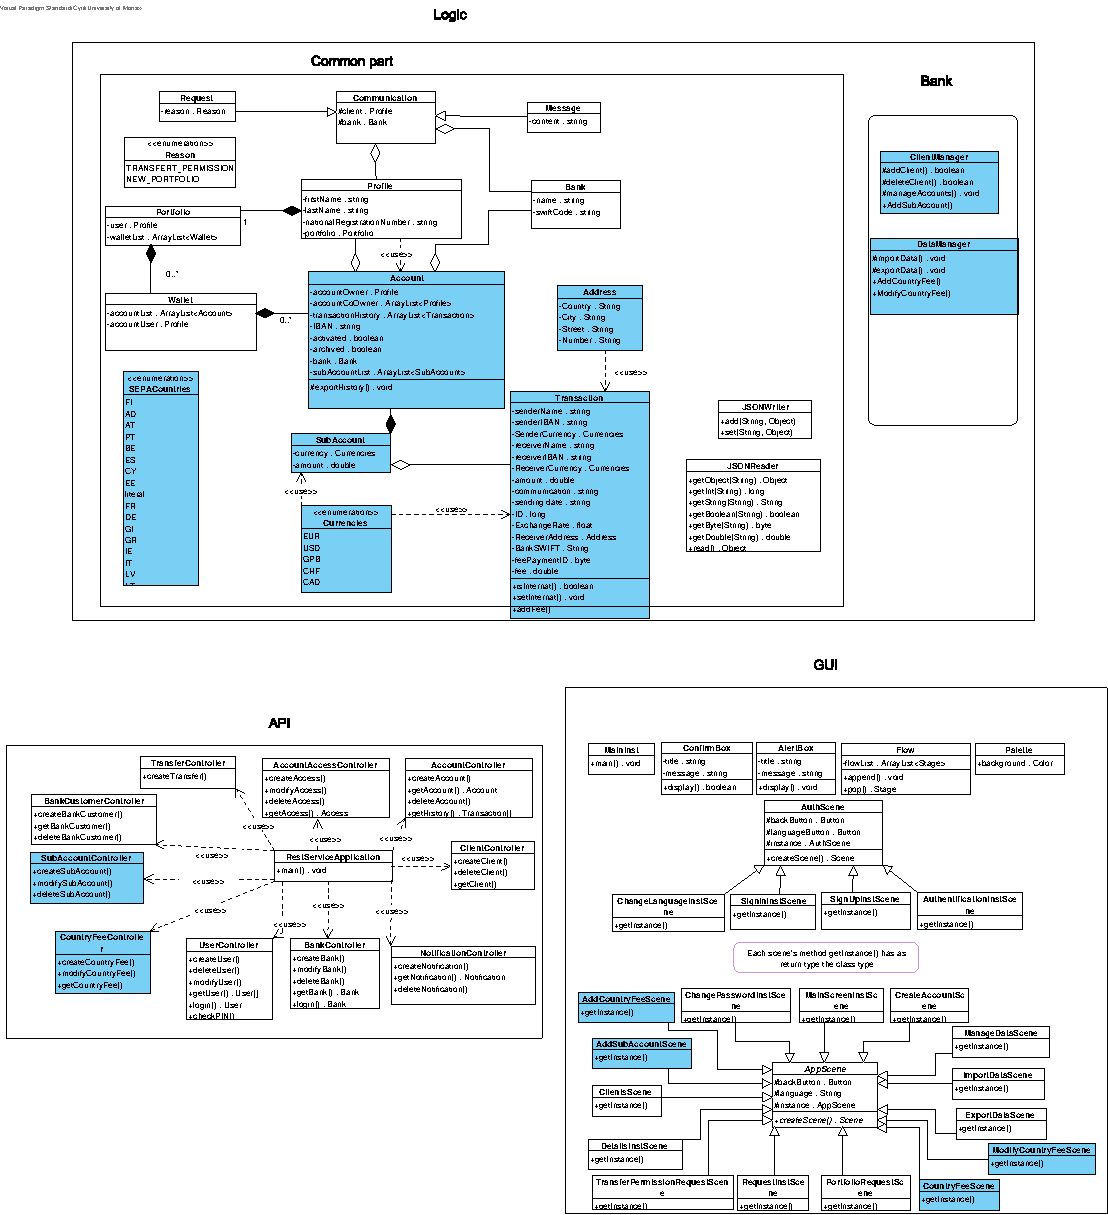
\includegraphics[width=\linewidth]{img/Class Diagram Institution - Extension 2.pdf}
	}
	\caption{Diagramme de classe de l'application service financier de l'extension 2}
\end{figure}
\subfile{subfiles/Class Institution - Extension 2.tex}
\newpage

\subsection{Sequence diagram}

\begin{figure}[h!]
	\hbox{
		\centering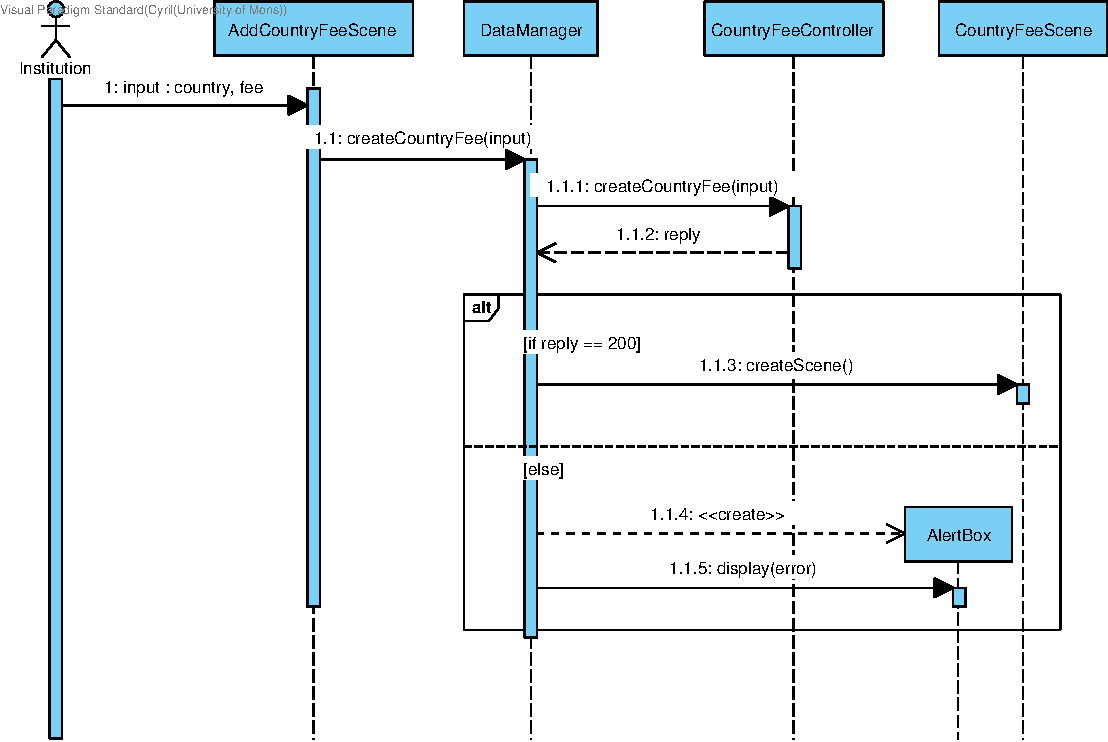
\includegraphics[width=\linewidth]{img/Sequence 4 - Extension 2.pdf}
	}
	\caption{Ajouter frais pour un pays}
	\end{figure}
	\subfile{subfiles/Sequence 4 - Extension 2.tex}
\newpage

\begin{figure}[h!]
	\hbox{
		\centering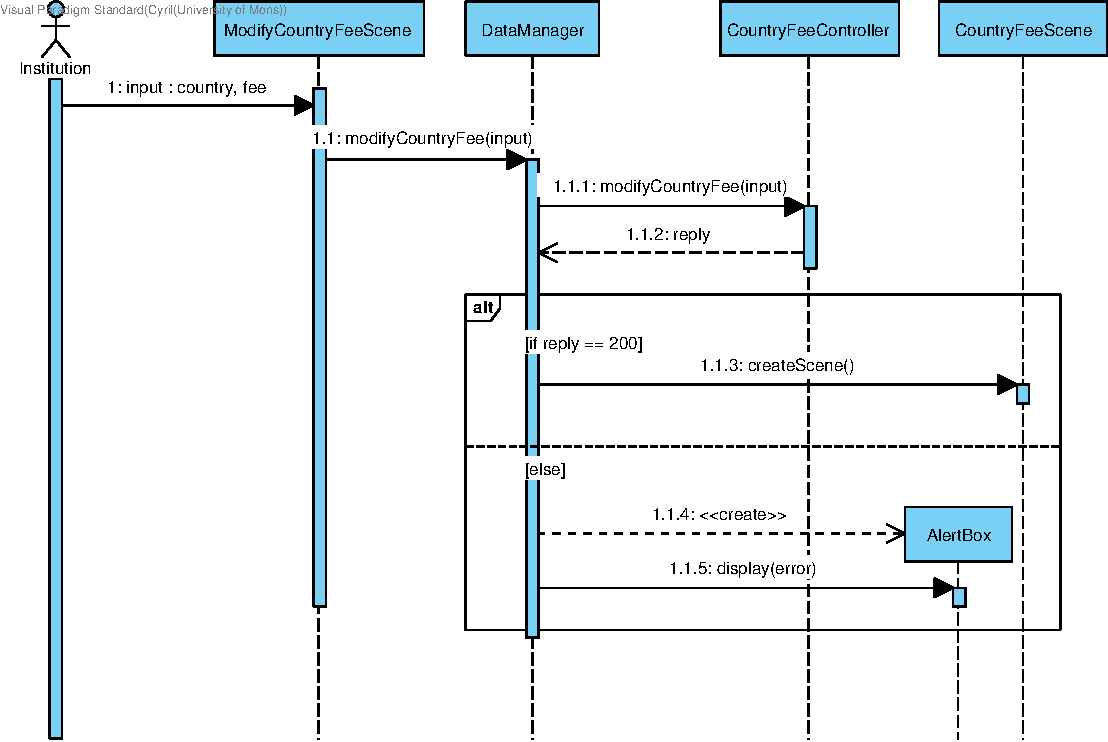
\includegraphics[width=\linewidth]{img/Sequence 5 - Extension 2.pdf}
	}
	\caption{Modifier frais pour un pays}
	\end{figure}
	\subfile{subfiles/Sequence 5 - Extension 2.tex}
\newpage

\begin{figure}[h!]
	\hbox{
		\centering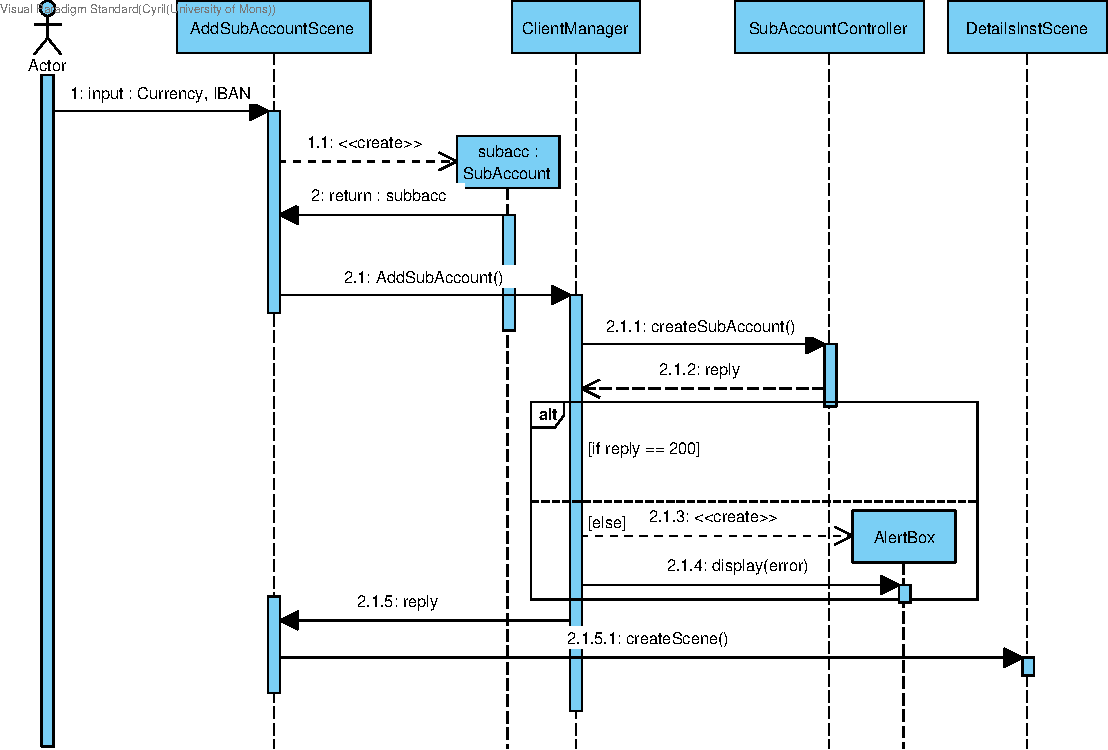
\includegraphics[width=\linewidth]{img/Sequence 6 - Extension 2.pdf}
	}
	\caption{Ajouter une devise pour un compte}
\end{figure}
\subfile{subfiles/Sequence 6 - Extension 2.tex}
\newpage

\section{Modèle de données}

\begin{figure}[h]
	\centering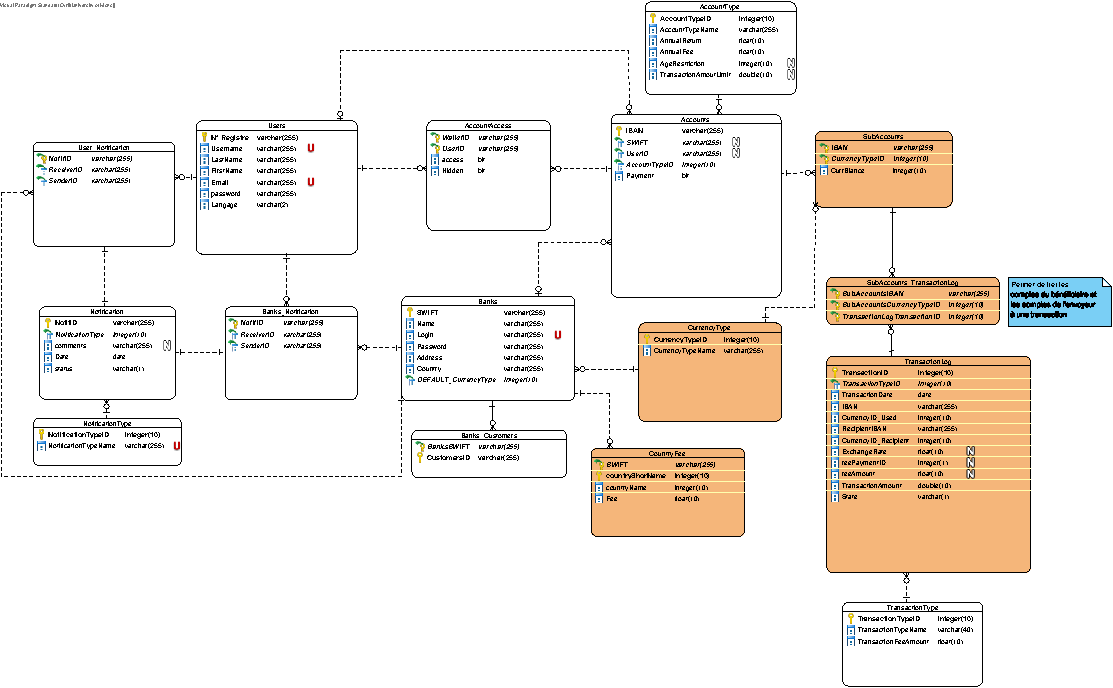
\includegraphics[width=\linewidth]{img/BDD - Extension 2.pdf}
	\caption{Diagramme d'entité relation de l'extension 2.}
\end{figure}
\subfile{subfiles/BDD - Extension 2.tex}

\newpage

\section{Maquette de l'interface de l'application client}

\subfile{subfiles/UI Client - Extension 2.tex}

\newpage

\section{Maquette de l'interface de l'application pour une institution}

\subfile{subfiles/UI Institution - Extension 2.tex}





\chapter{Extension C : Gestion des contrats d’assurance - François \textsc{Vion}}



\newpage



\section{Diagrammes de conception UML : application client}



\subsection{Use case diagram}

\subfile{subfiles/Use Case Client Assurance.tex}

\newpage

\subsection{Interaction overview diagram}

\subfile{subfiles/Interaction Overview Client Assurance.tex}

\newpage

\subsection{Class diagram}

\subfile{subfiles/Class Client Assurance.tex}

\newpage

\subsection{Sequence diagram}

\subfile{subfiles/Sequence Diagram Client Assurance.tex}

\newpage



\section{Diagrammes de conception UML : application institution}



\subsection{Use case diagram}

\subfile{subfiles/Use Case Bank Assurance.tex}

\newpage

\subsection{Interaction overview diagram}

\subfile{subfiles/Interaction Overview Diagram Bank Assurance.tex}

\newpage

\subsection{Class diagram}

\subfile{subfiles/Class Bank Assurance.tex}

\newpage

\subsection{Sequence diagram}

\paragraph{}Le seul diagramme de séquence de cette partie (Envoyer un devis) pouvant être réalisé sous la forme d’un fonctionnement type tel que décrit dans les diagrammes de séquence de la partie commune, celui-ci ne sera pas décrit. Il s’agit en effet de la création d’un objet via les entrées d’un utilisateur afin d’être ajoutées par après dans la base de données via l’API (deuxième diagramme type).

\newpage

\section{Modèle de données}

\subfile{subfiles/BDD Assurance.tex}

\newpage

\section{Maquette de l'interface utilisateur et institution}

\subfile{subfiles/UI Assurance.tex}

\newpage




\chapter{Extension D : Paiements et gestion de fraudes - Arnaud \textsc{Moreau}}





\newpage




\section{Diagrammes de conception UML : application client}




\subsection{Use case diagram}

\begin{figure}[h!]
%\vspace{2cm}
\hspace{-1cm}
\hbox{
	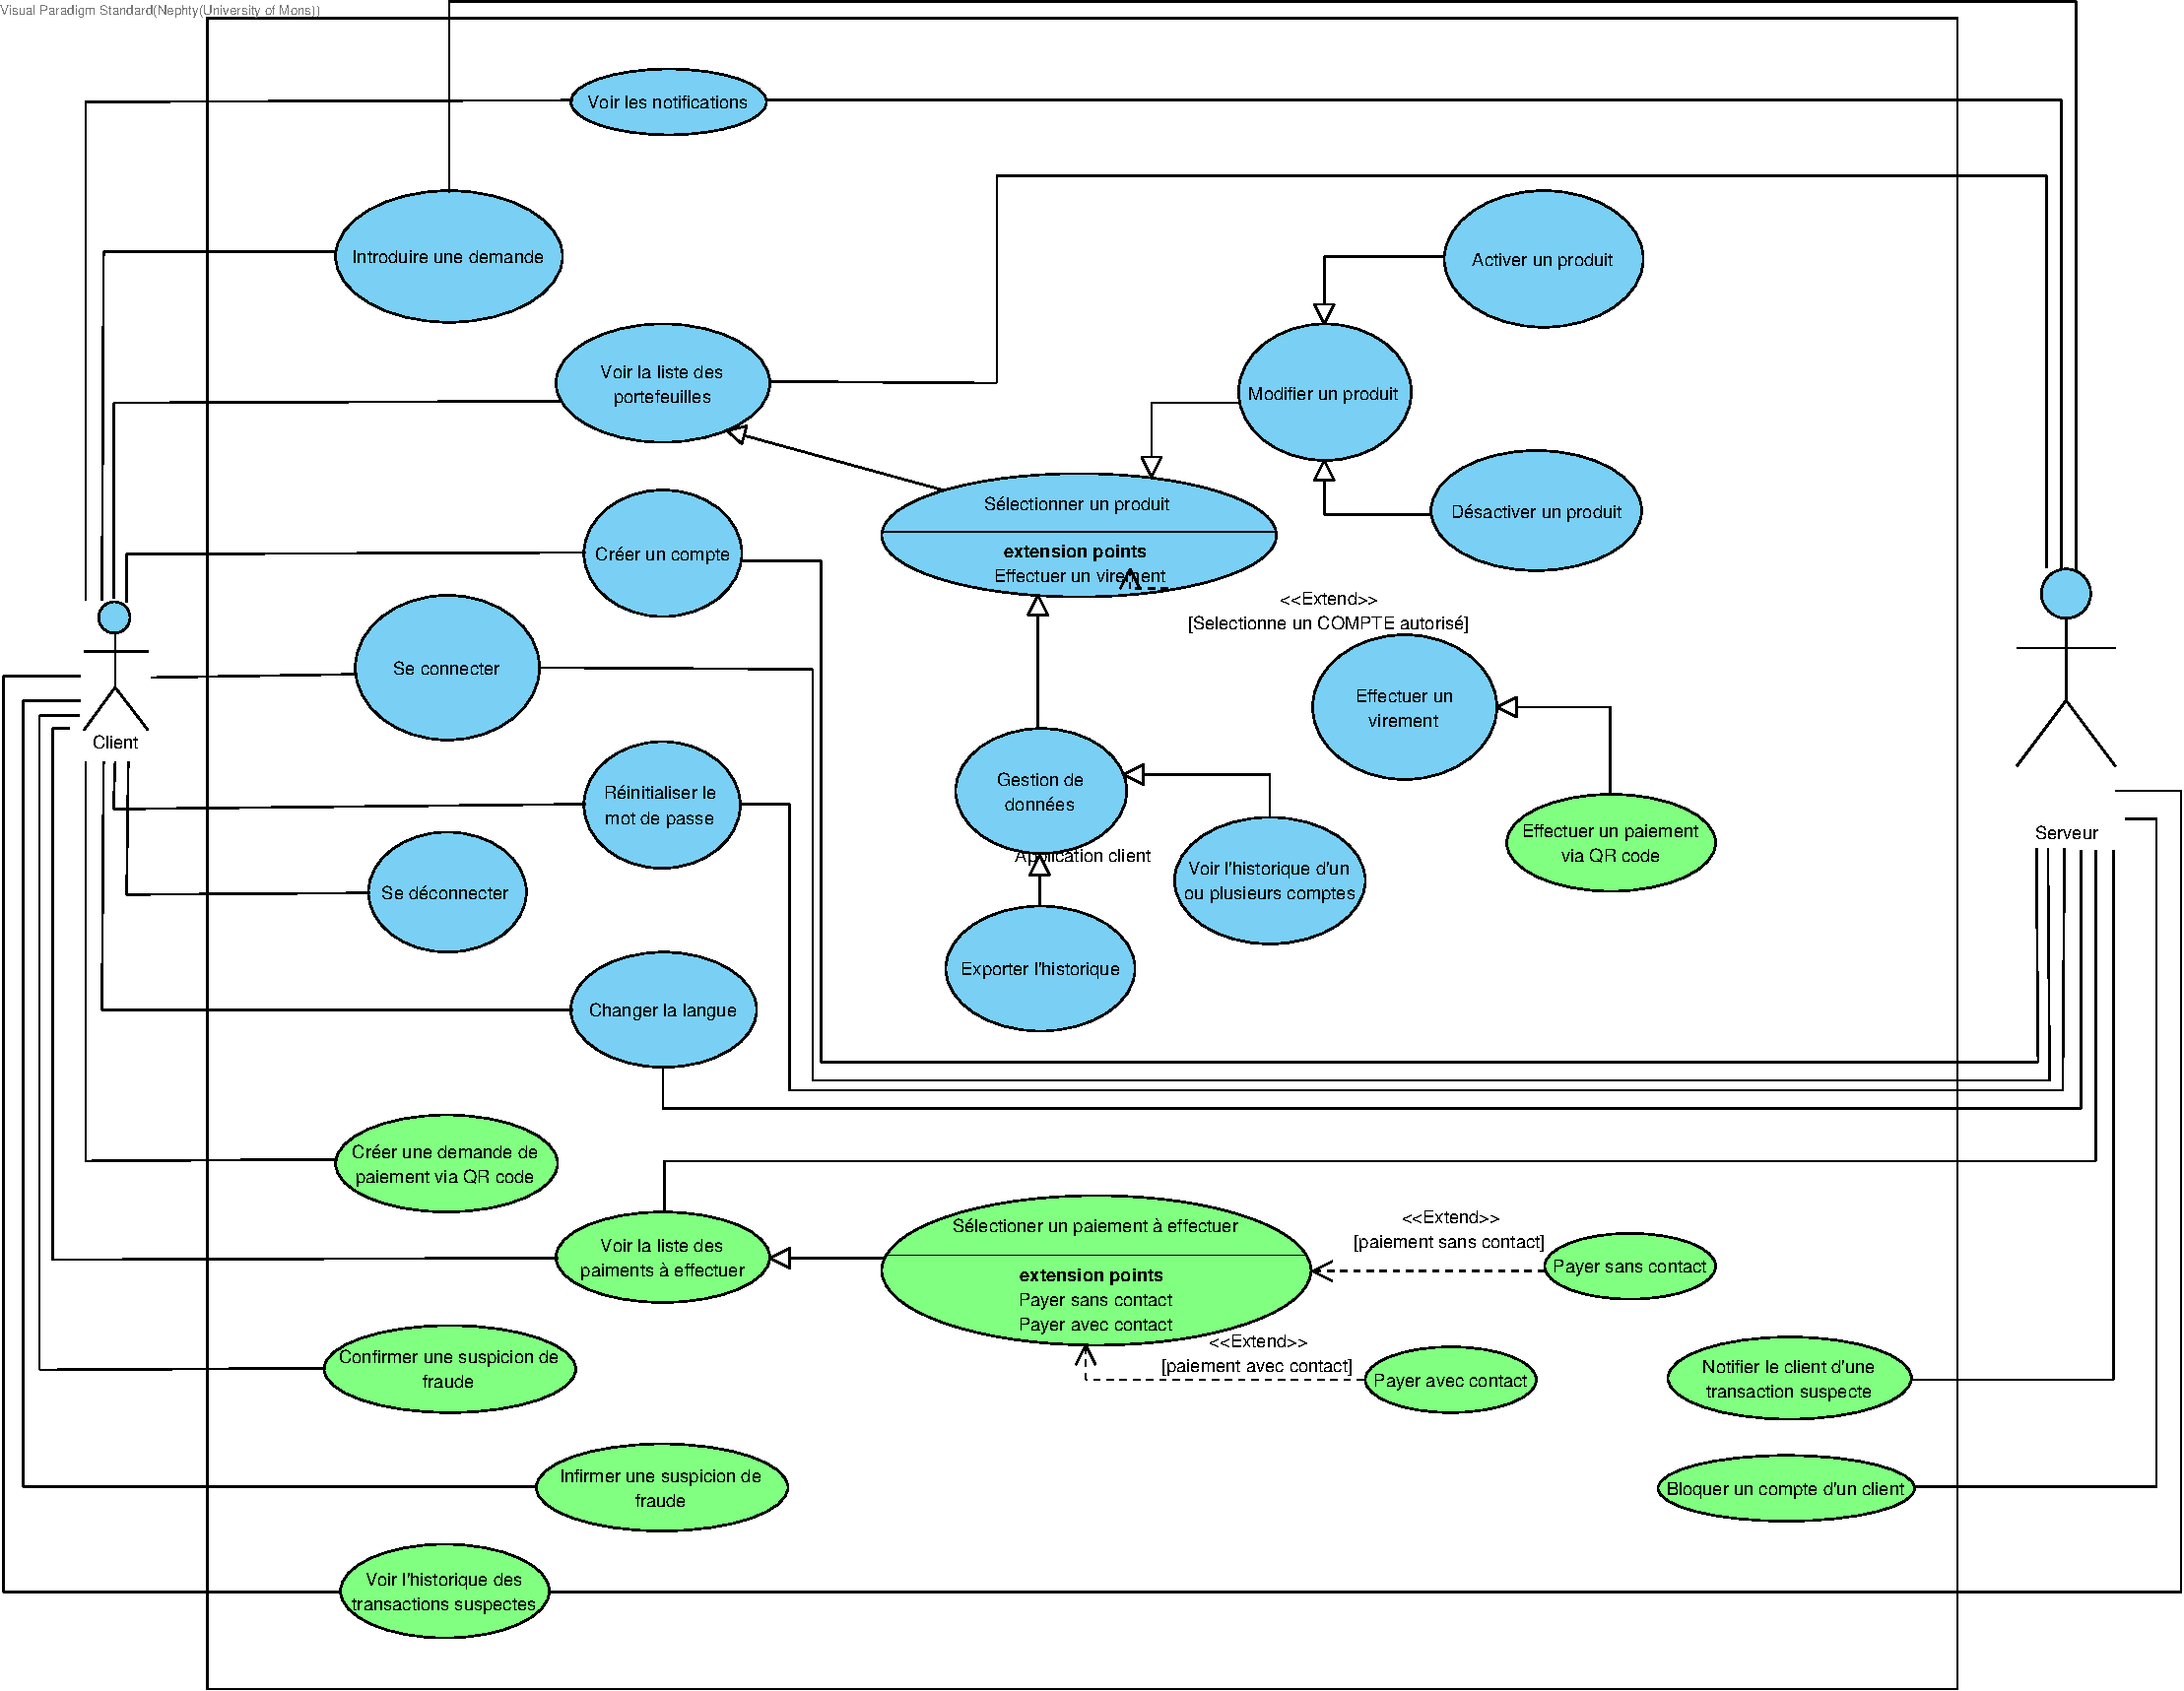
\includegraphics[scale=0.45]{img/Use Case Client - Extension 6.pdf}
}
\caption{Nouveau diagramme de cas d'utilisation de l'application client}
\end{figure}

\subfile{subfiles/Use Case Client - Extension 6.tex}

\newpage

\subsection{Interaction overview diagram}

\subfile{subfiles/Interaction Overview Client - Extension 6.tex}

\begin{figure}[h!]
\hspace{-3cm}
\hbox{
	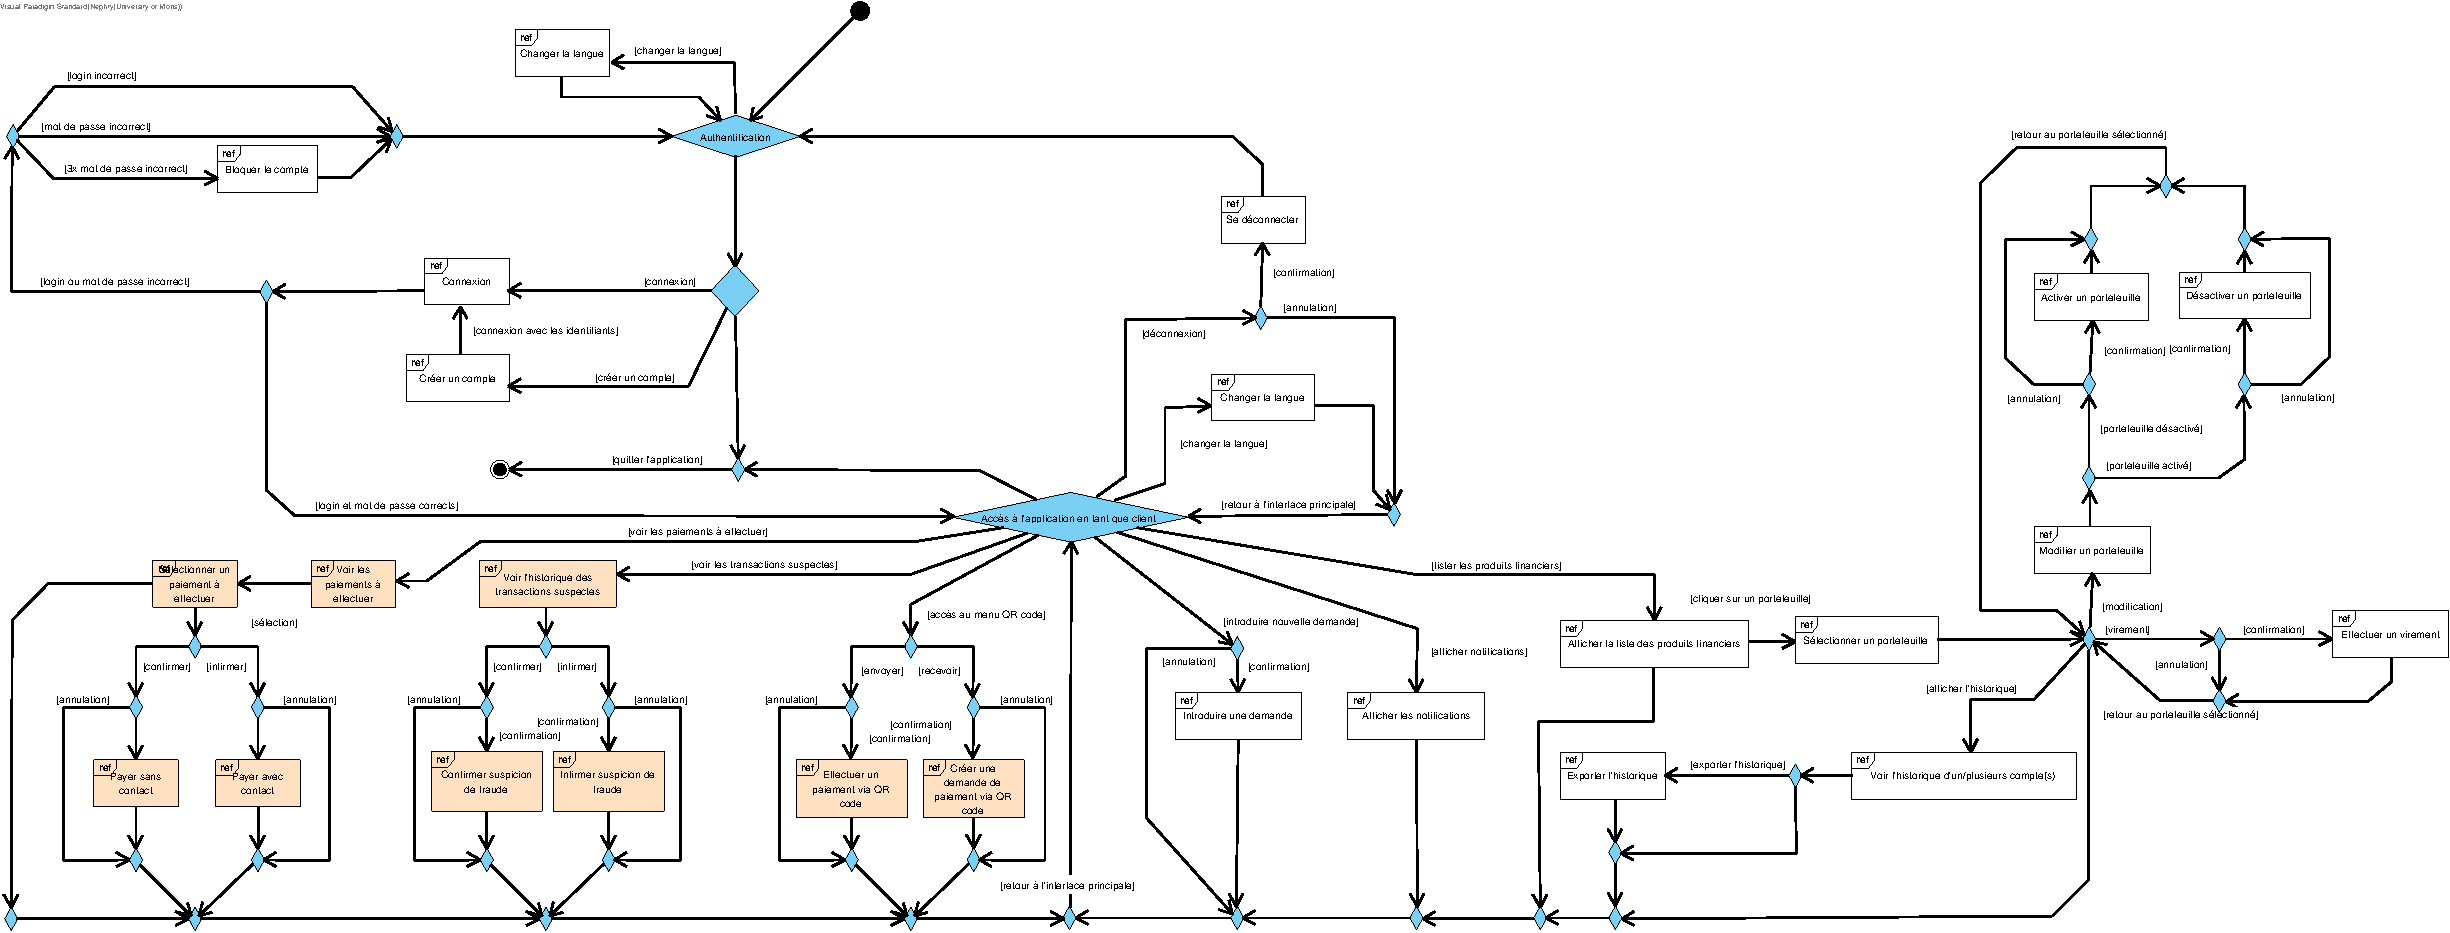
\includegraphics[scale=0.5]{img/Interaction Overview Client - Extension 6.pdf}
}
\caption{Nouveau diagramme d'interaction de l'application client}
\end{figure}

\newpage

\subsection{Class diagram}

\subfile{subfiles/Class Client - Extension 6.tex}

\begin{figure}[h!]
\hspace{1.25cm}
\hbox{
	\centering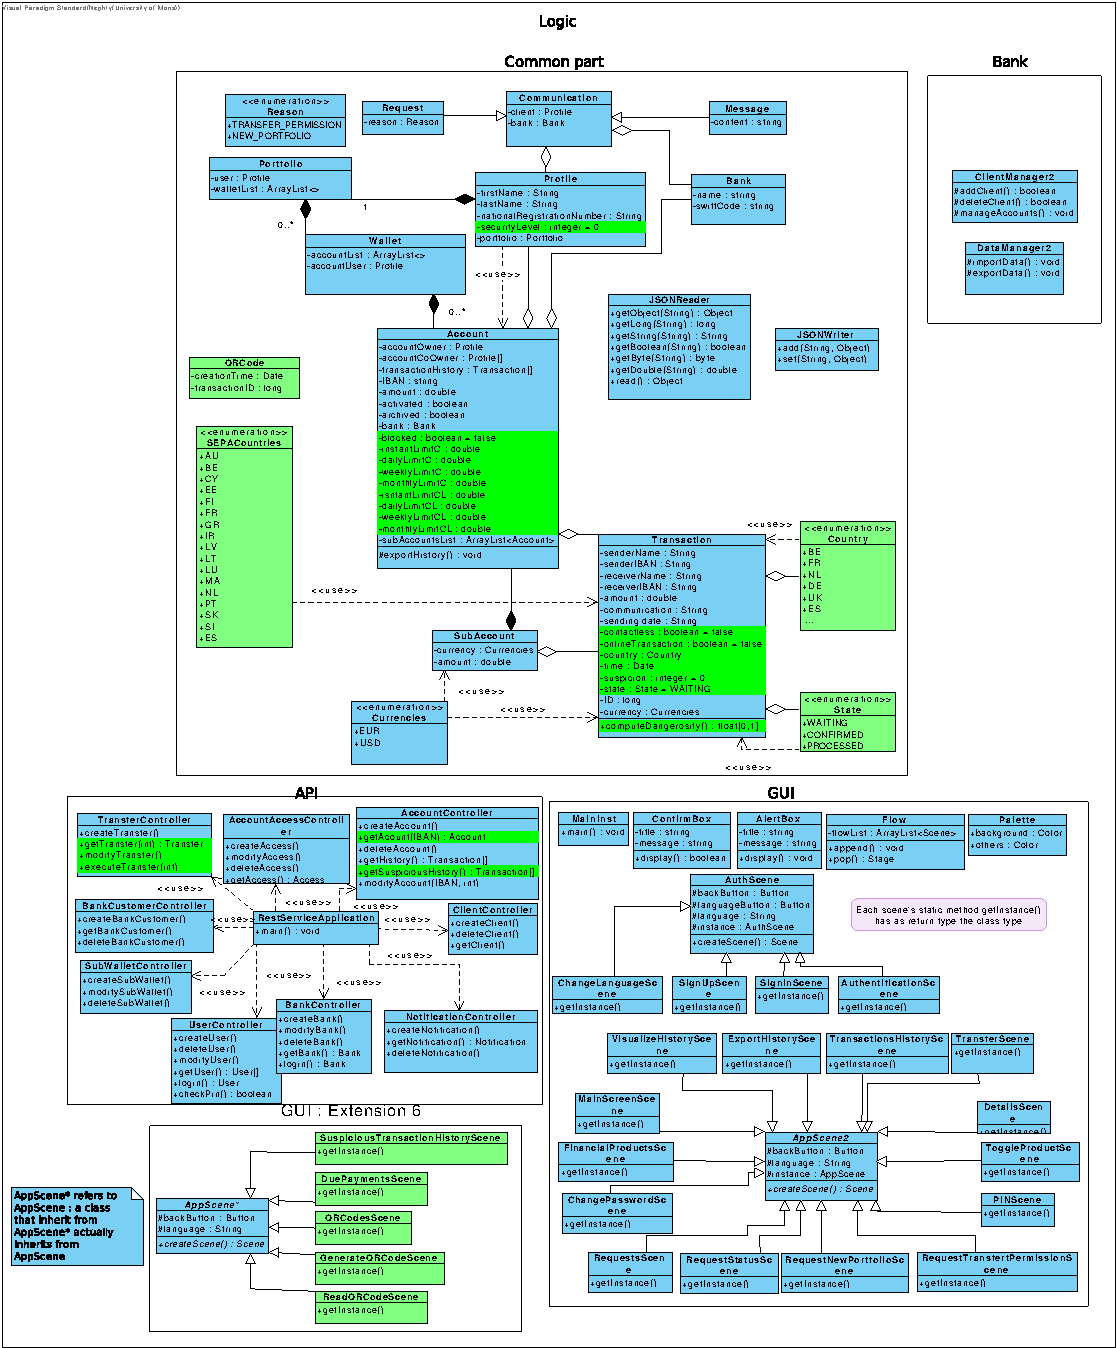
\includegraphics[scale=0.6]{img/Class Client - Extension 6.pdf}
}
\caption{Nouveau diagramme de classes de l'application client}
\end{figure}

\newpage

\subsection{Sequence diagram}

\begin{figure}[h!]
\hbox{
    \centering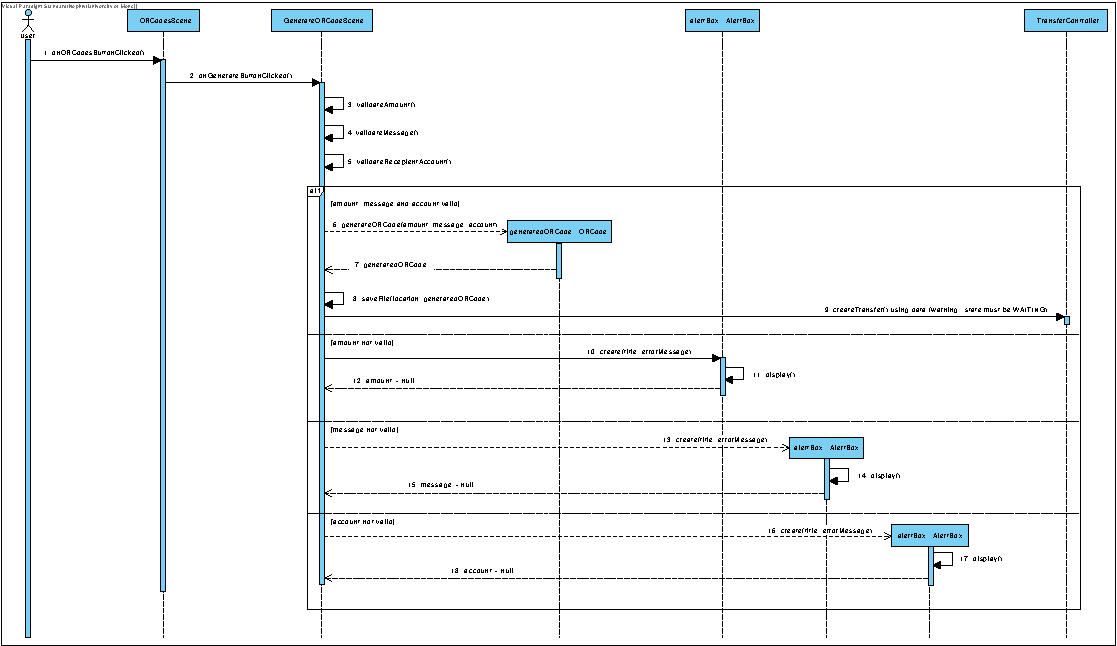
\includegraphics[width=\linewidth]{img/Sequence 1 - Extension 6.pdf}
}
\caption{Créer une demande de paiement via QR code}
\end{figure}

\subfile{subfiles/Sequence 1 - Extension 6.tex}

\newpage

\begin{figure}[h!]
\hbox{
    \centering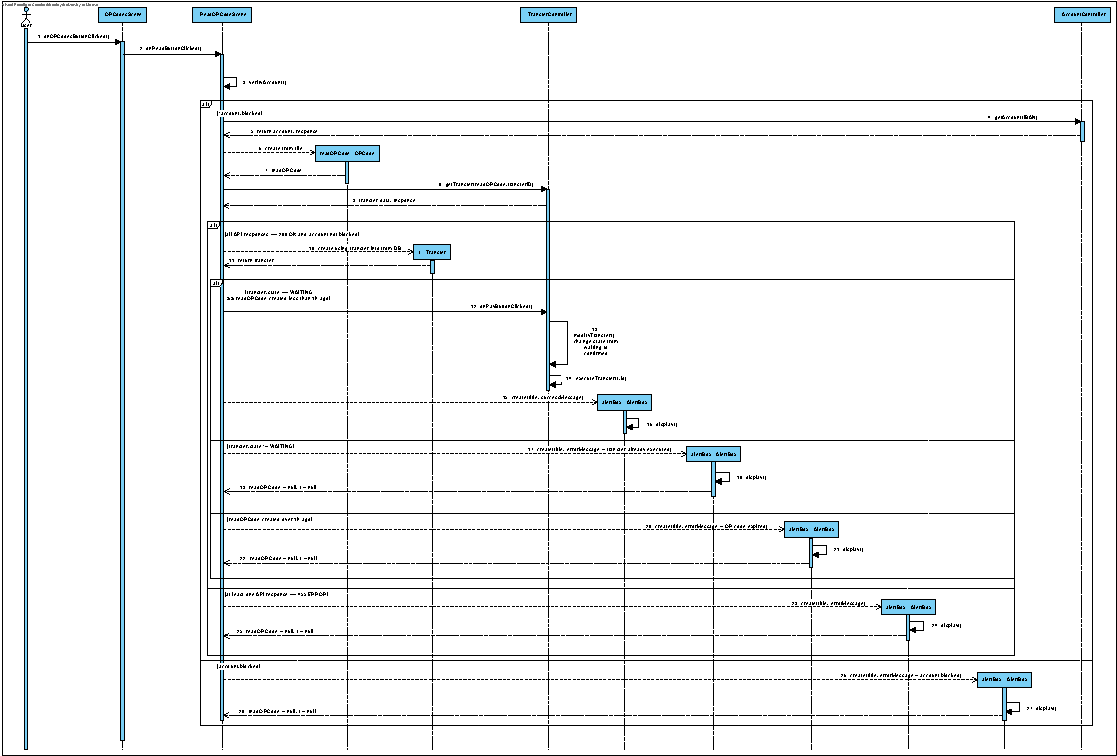
\includegraphics[width=\linewidth]{img/Sequence 2 - Extension 6.pdf}
}
\caption{Effectuer un paiement via QR code}
\end{figure}

\subfile{subfiles/Sequence 2 - Extension 6.tex}

\newpage

\begin{figure}[h!]
\hbox{
    \centering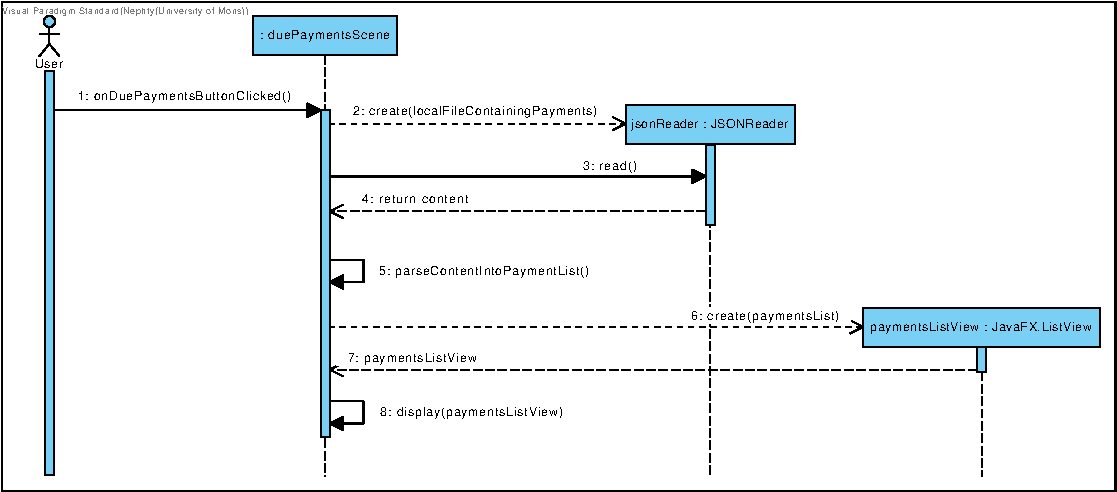
\includegraphics[width=\linewidth]{img/Sequence 3 - Extension 6.pdf}
}
\caption{Voir la liste des paiements à effectuer}
\end{figure}

\subfile{subfiles/Sequence 3 - Extension 6.tex}

\newpage

\begin{figure}[h!]
\hbox{
    \centering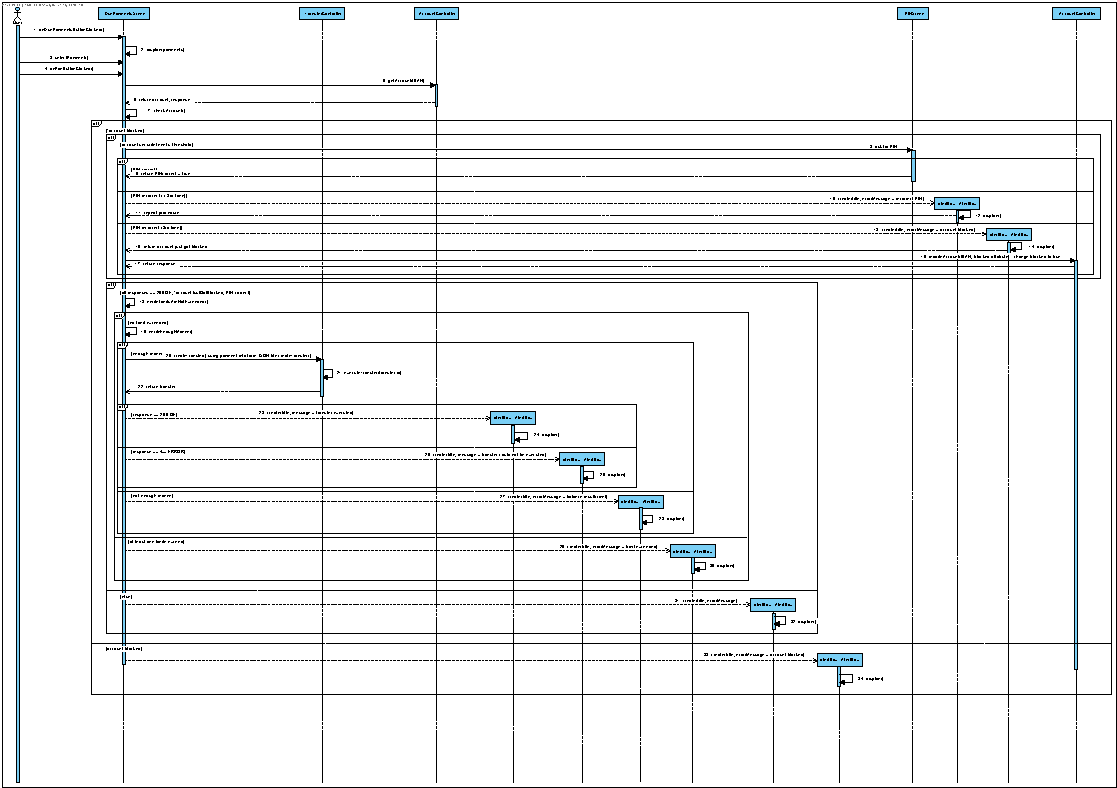
\includegraphics[width=\linewidth]{img/Sequence 4 - Extension 6.pdf}
}
\caption{Payer sans contact}
\end{figure}

\subfile{subfiles/Sequence 4 - Extension 6.tex}

\newpage

\begin{figure}[h!]
\hbox{
    \centering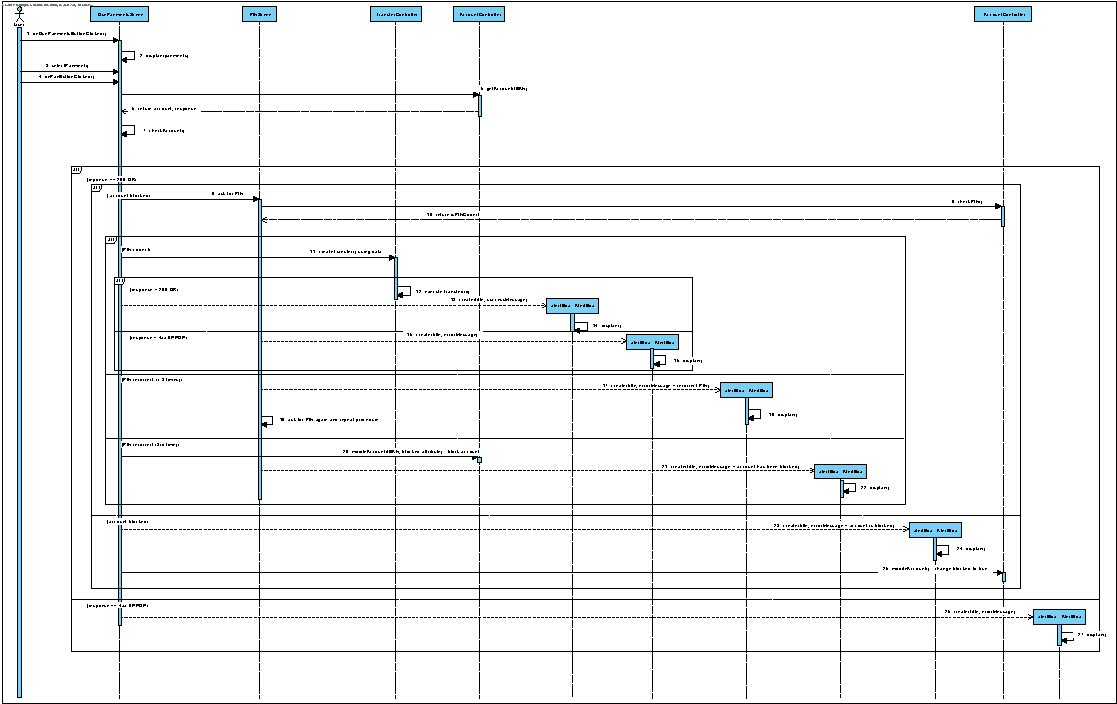
\includegraphics[width=\linewidth]{img/Sequence 5 - Extension 6.pdf}
}
\caption{Payer avec contact}
\end{figure}

\subfile{subfiles/Sequence 5 - Extension 6.tex}

\newpage

\begin{figure}[h!]
\hbox{
    \centering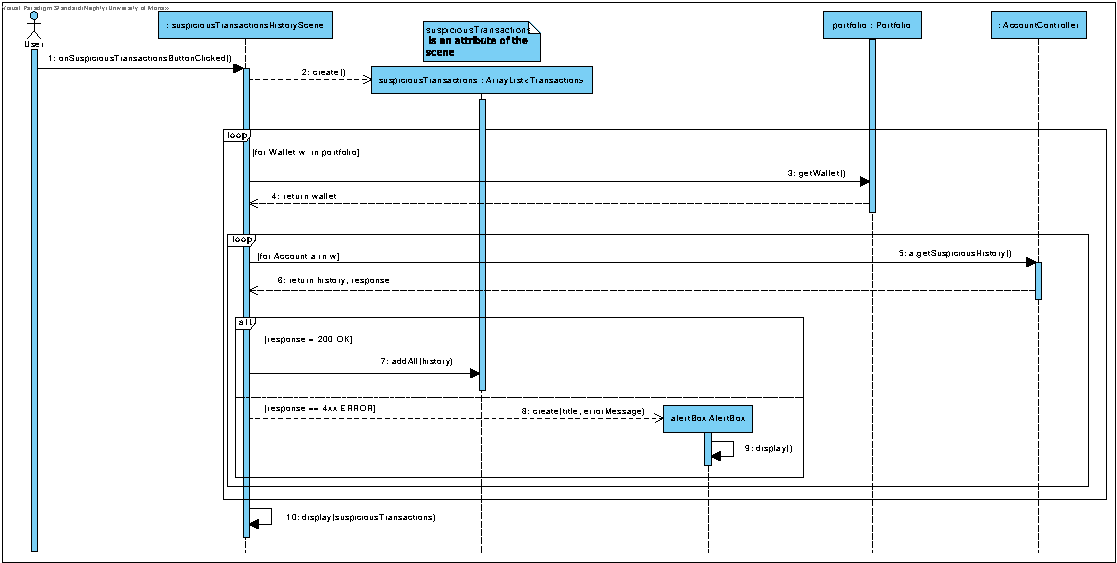
\includegraphics[width=\linewidth]{img/Sequence 6 - Extension 6.pdf}
}
\caption{Voir l'historique des transactions suspectes}
\end{figure}

\subfile{subfiles/Sequence 6 - Extension 6.tex}

\newpage

\begin{figure}[h!]
\hbox{
    \centering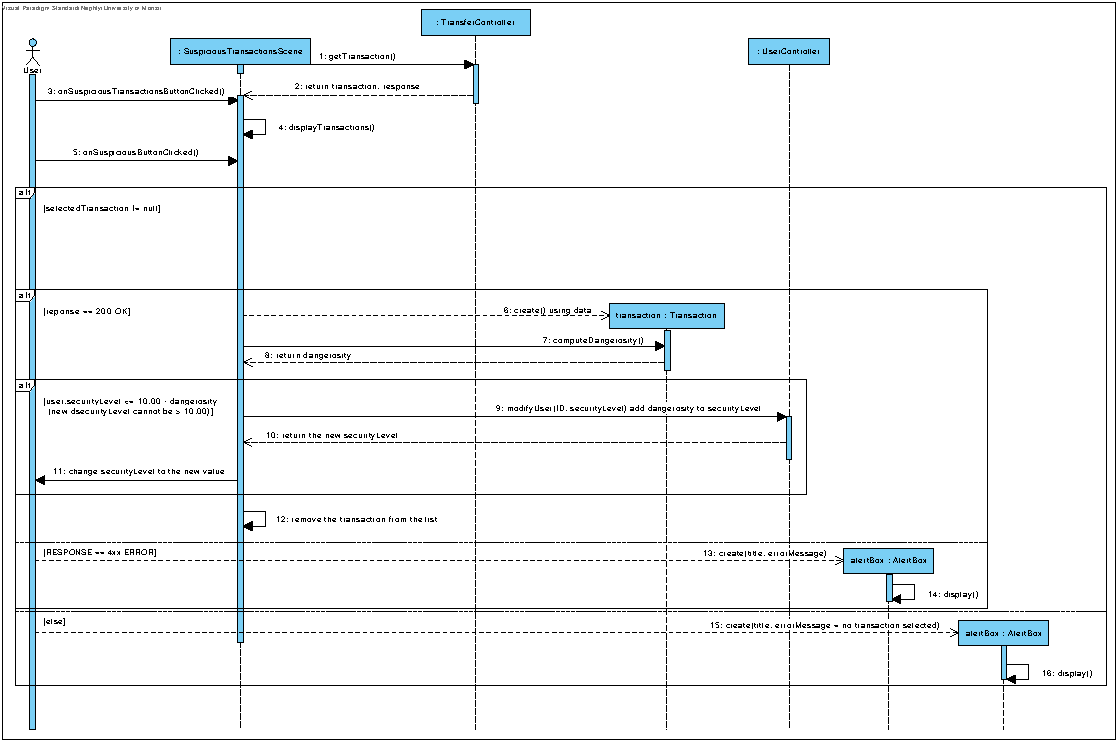
\includegraphics[width=\linewidth]{img/Sequence 7 - Extension 6.pdf}
}
\caption{Confirmer une suspicion de fraude}
\end{figure}

\subfile{subfiles/Sequence 7 - Extension 6.tex}

\newpage

\begin{figure}[h!]
\hbox{
    \centering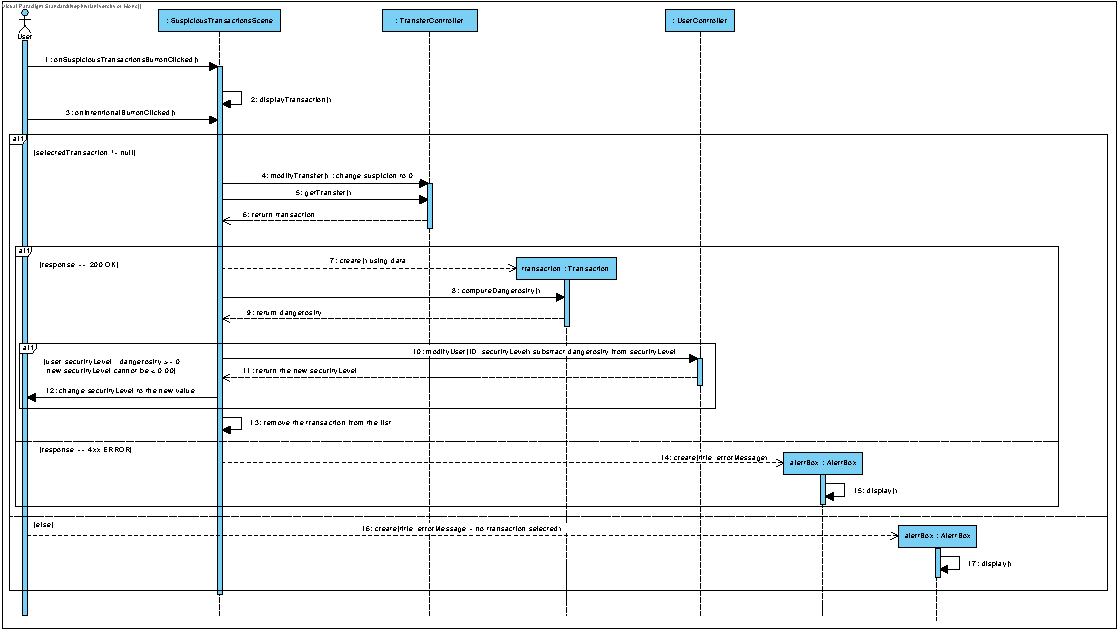
\includegraphics[width=\linewidth]{img/Sequence 8 - Extension 6.pdf}
}
\caption{Infirmer une suspicion de fraude}
\end{figure}

\subfile{subfiles/Sequence 8 - Extension 6.tex}

\newpage

\begin{figure}[h!]
\hbox{
	\centering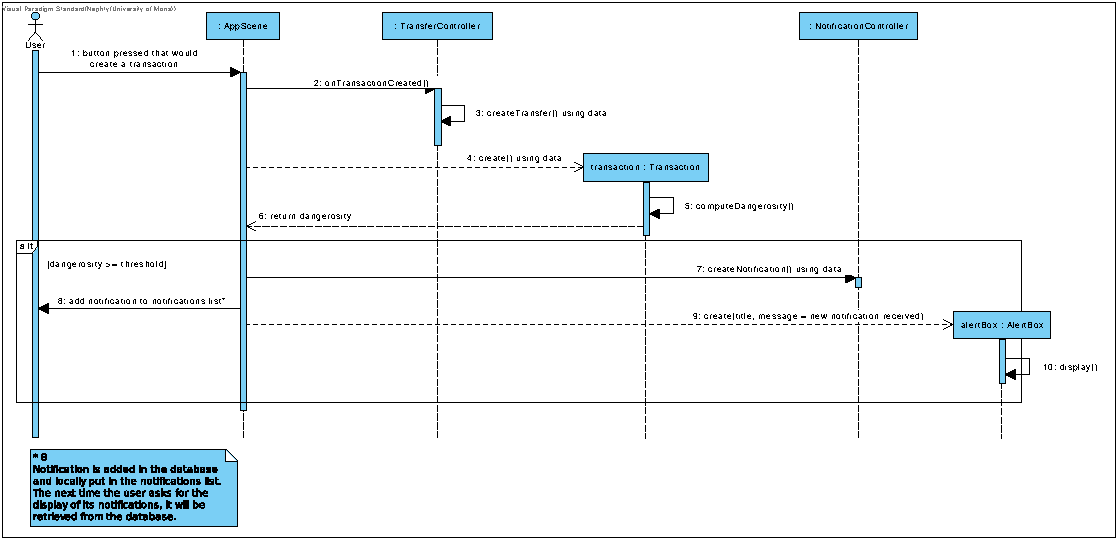
\includegraphics[width=\linewidth]{img/Sequence 9 - Extension 6.pdf}
}
\caption{Notifier le client d'une transaction suspecte}
\end{figure}
	
\subfile{subfiles/Sequence 9 - Extension 6.tex}
	

\newpage




\section{Diagrammes de conception UML : application institution}




\subsection{Use case diagram}

\begin{figure}[h!]
\hbox{
	\centering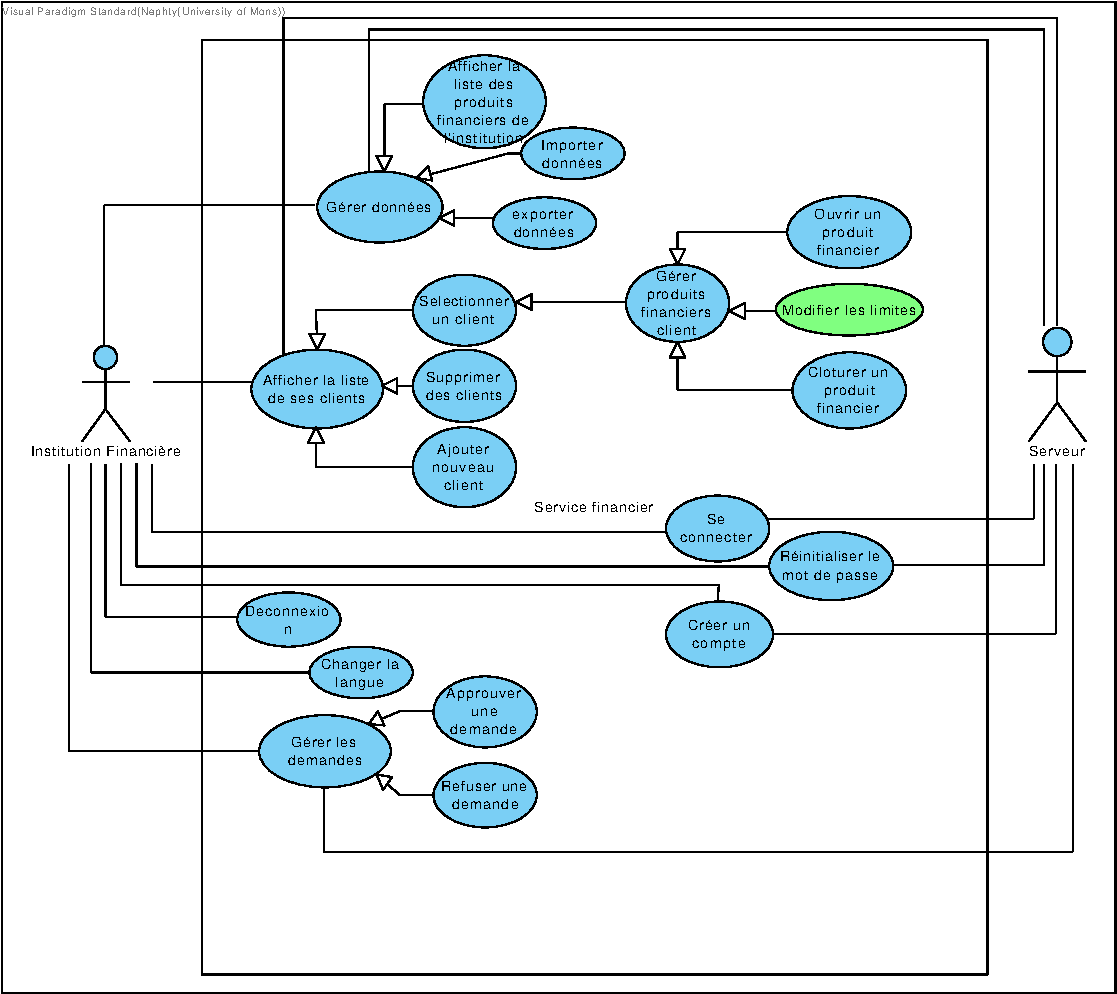
\includegraphics[width=\linewidth]{img/Use Case Institution - Extension 6.pdf}
}
\end{figure}

\subfile{subfiles/Use Case Institution - Extension 6.tex}

\newpage

\subsection{Interaction overview diagram}

\subfile{subfiles/Interaction Overview Institution - Extension 6.tex}

\begin{figure}[h!]
\hbox{
	\centering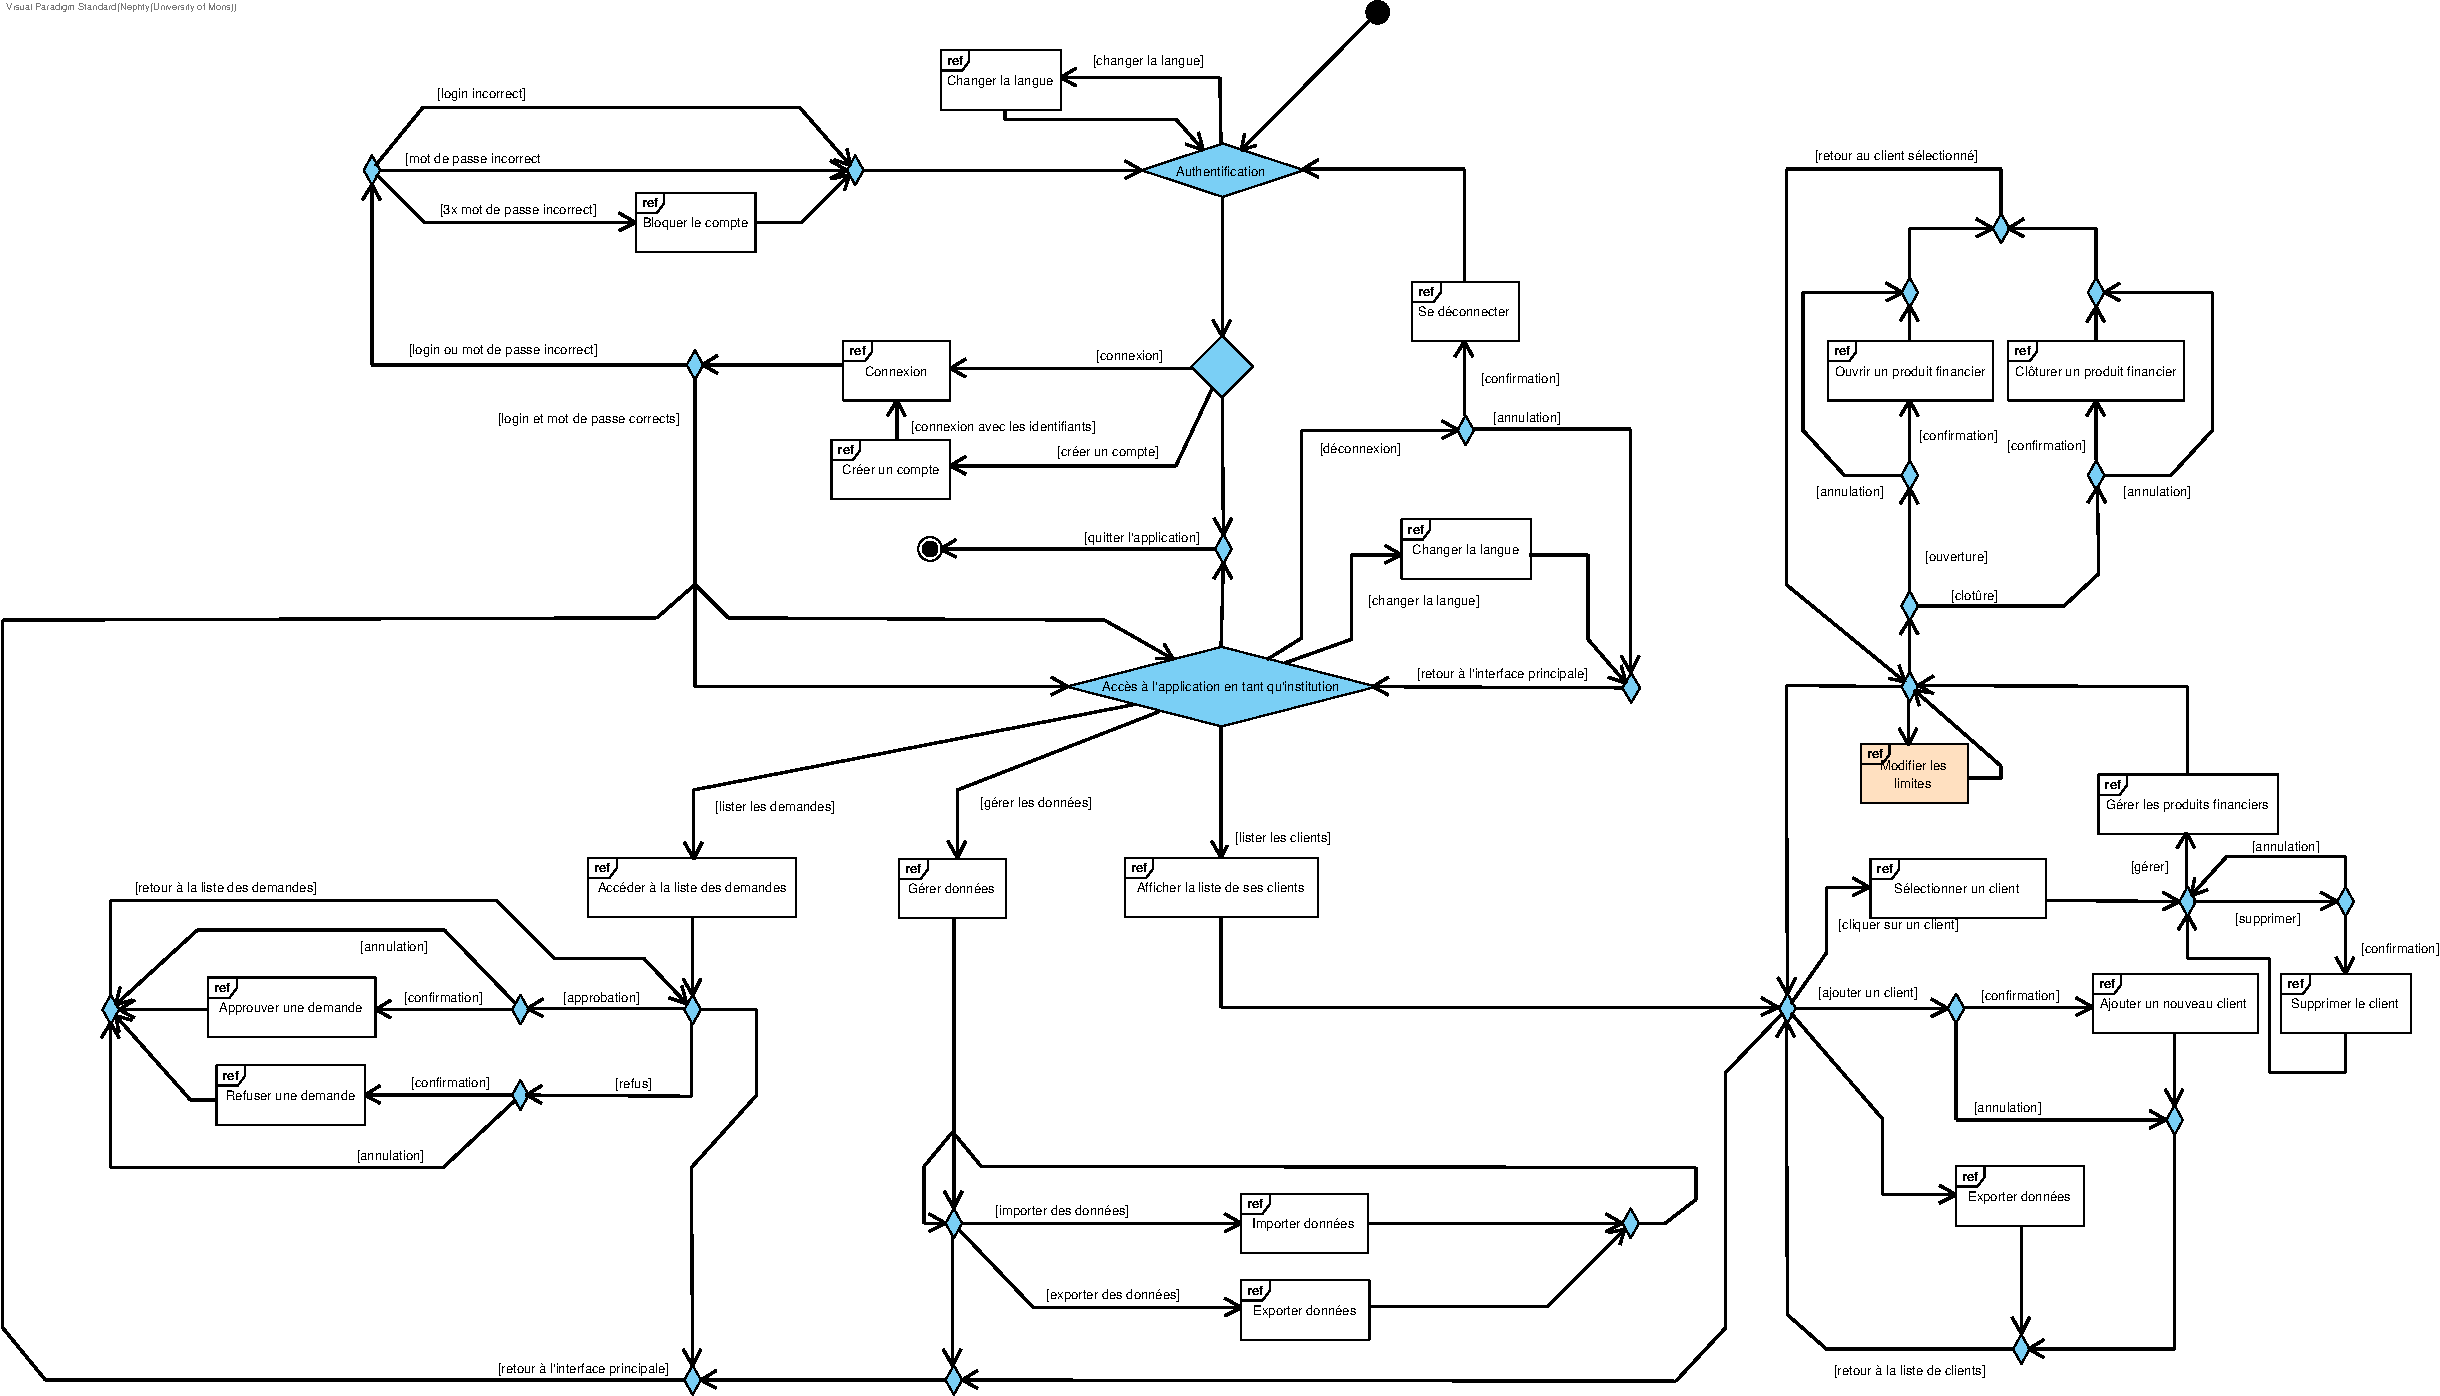
\includegraphics[scale=0.33]{img/Interaction Overview Institution - Extension 6.pdf}
}
\end{figure}

\newpage

\subsection{Class diagram}

\subfile{subfiles/Class Institution - Extension 6.tex}

\begin{figure}[h!]
\hbox{
	\centering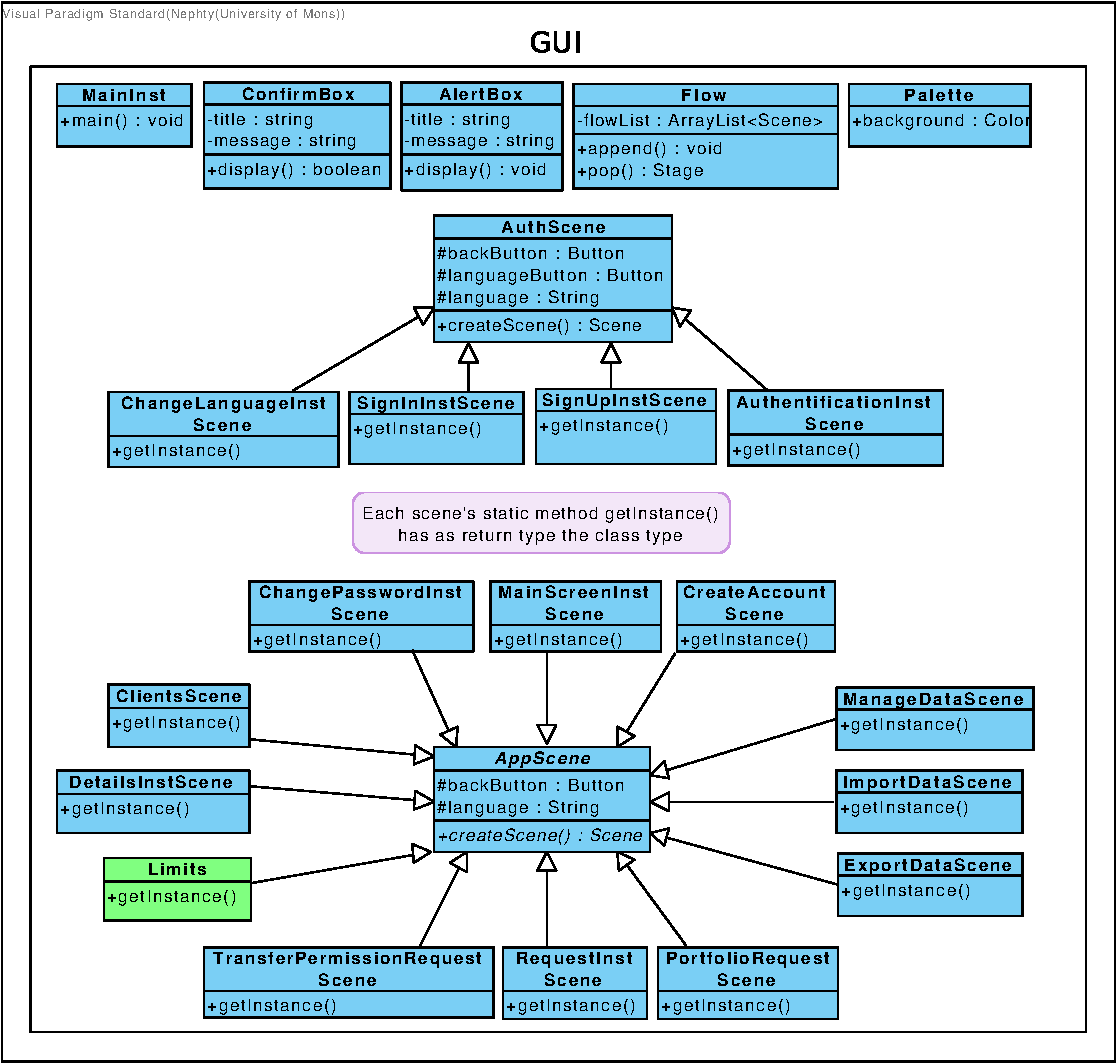
\includegraphics[width=\linewidth]{img/Class Institution - Extension 6.pdf}
}
\end{figure}

\newpage

\subsection{Sequence diagram}


\begin{figure}[h!]
\hbox{
    \centering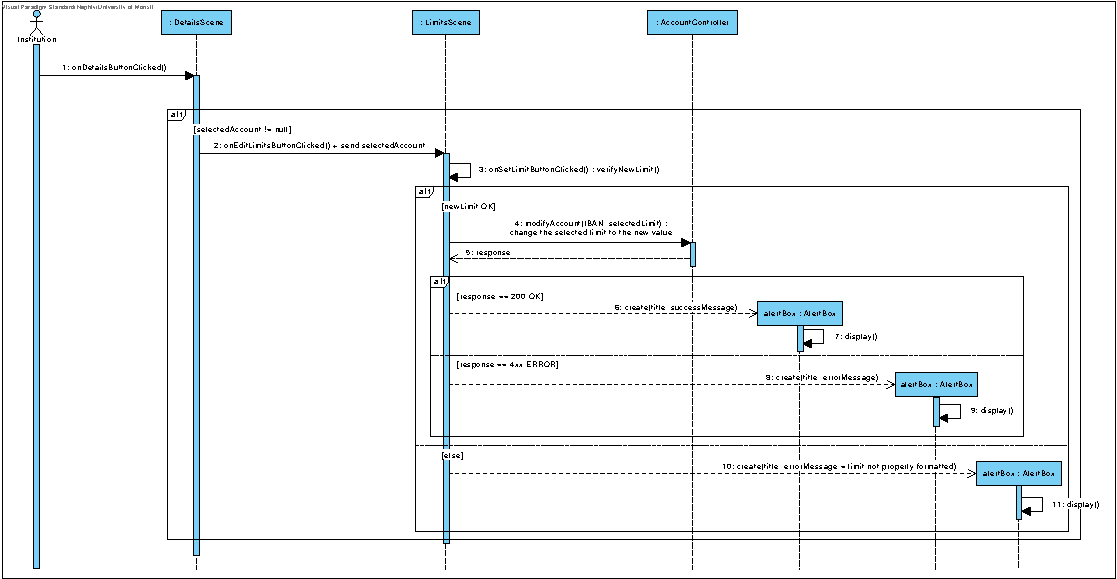
\includegraphics[width=\linewidth]{img/Sequence 10 - Extension 6.pdf}
}
\caption{Notifier le client d'une transaction suspecte}
\end{figure}

\subfile{subfiles/Sequence 10 - Extension 6.tex}

\newpage




\section{Modèle de données}

\subfile{subfiles/Modele de donnees - Extension 6.tex}

%\vspace{1cm}
\begin{figure}[h!]
\hspace{0.75cm}
\hbox{
	\centering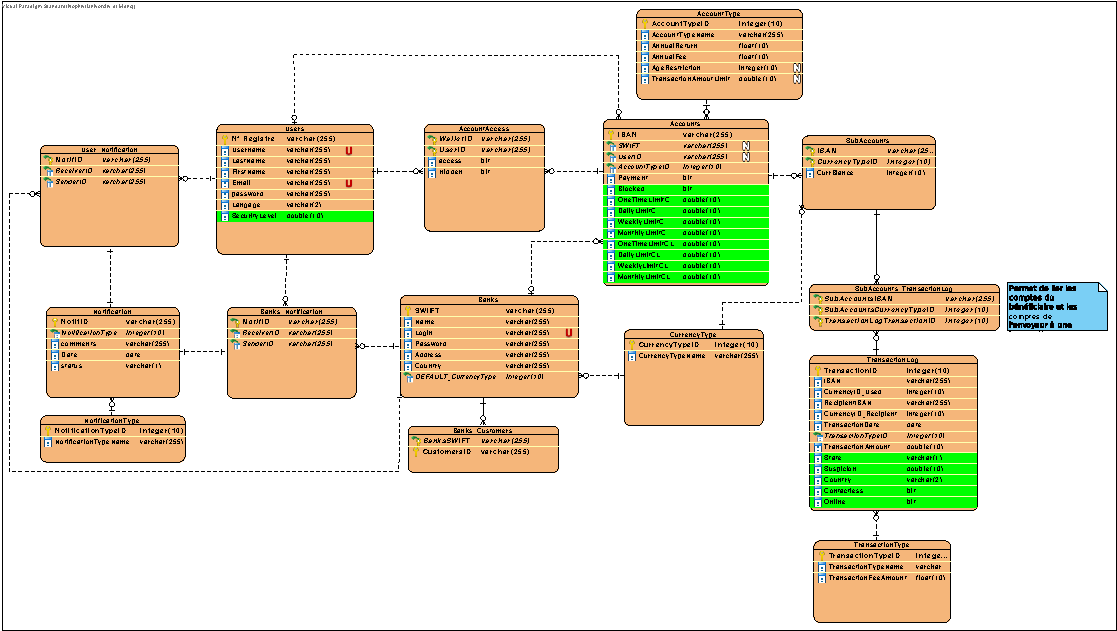
\includegraphics[scale=0.69]{img/Entity Relation - Extension 6.pdf} % nice
}
\end{figure}

\newpage




\section{Maquette de l'interface utilisateur}

\subfile{subfiles/UI Client - Extension 6.tex}

\vspace*{\fill}

\paragraph{Illustration du diagramme} Par souci de clareté, ce diagramme est disponible en annexe du rapport.

\newpage


\section{Maquette de l'interface institution}

\subfile{subfiles/UI Institution - Extension 6.tex}

\vspace*{\fill}

\paragraph{Illustration du diagramme} Par souci de clareté, ce diagramme est disponible en annexe du rapport.




\end{document}
